% Kapitel 2 - Related Work / Literaturanalyse
\section{Theoretical Background}\label{sec:RelatedWork}

%\subsection{The New Paradigm: The Automotive Interior as an Interaction Space/The New Paradigm of the Automotive Interior}
% This section sets the stage. It establishes the "why" the fundamental shift in the automotive world that makes my research relevant.
The field of Human-Vehicle Interaction (\gls{HVI}) is currently undergoing a dramatic transformation, driven by two intertwined dimensions: rapid advancements in infotainment technology and a fundamental rethinking of vehicle interior design \cite{khorsandi_fabricar_2023}. These concurrent developments create a critical opportunity to revisit our established notions of in-car interaction and how an interactive moving space is perceived \cite{khorsandi_fabricar_2023}. At the heart of this paradigm shift is the steady advance of vehicle automation. As automation technology matures, it promises to fundamentally alter the occupant's role from that of an active driver to a passenger \cite{detjen_how_2021}, redefining the vehicle itself from a pure modality of transport into a versatile 'living space' \cite{schartmuller_automated_2020}.

%\subsubsection{The Advent of Automated Driving}
\subsection{Automated Driving and Vehicle Interiors}
% Discuss the transition to highly automated driving (SAE Levels 3+) as an expected near-future reality.
% Definition of the SAE Levels
% Explain how this shifts the human's role from a driver to a passenger, freeing up attention from the primary driving task. 
% Definition of Driving Tasks

\begin{comment}   
The prospect of highly automated driving (HAD) is rapidly transitioning from a futuristic concept to a tangible reality, with a general consensus that it will be available in production vehicles in the near future \cite{pfleging_investigating_2016}.
% While various uncertainties remain, the scenario of driverless cars now appears as a possible, close future \cite{lipson_driverless_2017, litman_autonomous_2024}. 
Highly automated cars will potentially be the first vehicles where the driver can fully disengage mentally and physically from the task of driving for a prolonged period of time (SAE International, 2021). \cite{wilson_non-driving_2022}
\end{comment}

\begin{comment}
The transition toward highly automated driving (HAD), corresponding to SAE automation levels 3 and above \cite{on-road_automated_driving_orad_committee_taxonomy_2021} (see Table \ref{tab:sae-levels}), is no longer a distant vision but an increasingly imminent development. With significant technological progress and growing industry investment such systems will soon become available in production vehicles in the near future \cite{pfleging_investigating_2016}. At these levels of automation, the vehicle assumes full control over driving functions under specific conditions, allowing the human occupant to disengage from the (primary and secondary) driving task both physically and mentally for extended periods of time \cite{on-road_automated_driving_orad_committee_taxonomy_2021}.
\end{comment}

The transition toward highly automated driving (\gls{HAD}) is rapidly progressing, with systems at SAE automation Levels 3 and above \cite{on-road_automated_driving_orad_committee_taxonomy_2021} (see Fig. \ref{fig:sae-levels}) increasingly seen as viable for near-future implementation in consumer vehicles \cite{lipson_driverless_2017, litman_autonomous_2024, pfleging_investigating_2016}. Following the definition of SAE J3016 \textit{Levels of Driving Automation} \cite{on-road_automated_driving_orad_committee_taxonomy_2021}, Level 3 (Conditional Driving Automation) systems can perform the entire dynamic driving task within specific operational design domains, but require the human to act as a fallback-ready user. Levels 4 and 5 go beyond this: Level 4 (High Driving Automation) does not require human intervention within its operational design domain, and Level 5 (Full Driving Automation) operates under all roadway and environmental conditions without any human input. 

\begin{figure} [h!]
    \centering
    \includegraphics[width=1\linewidth]{images/SAE Levels.png}
    \caption{Levels of driving automation, based on SAE J3016 \cite{on-road_automated_driving_orad_committee_taxonomy_2021}}.
    \label{fig:sae-levels}
\end{figure}

\begin{comment}
   \begin{table}[h!]
\centering
\caption{Based on SAE J3016 Levels of Driving Automation \cite{on-road_automated_driving_orad_committee_taxonomy_2021}}
\label{tab:sae-levels}
\begin{tabular}{|c|l|p{8cm}|}
\hline
\textbf{SAE Level} & \textbf{Name} & \textbf{Description} \\
\hline
\textbf{0} & No Driving Automation & The human driver performs all aspects of the dynamic driving task (DDT). Systems may provide warnings but do not provide sustained vehicle control. \\
\hline
\textbf{1} & Driver Assistance & The system provides sustained assistance for \textit{either} lateral (steering) \textit{or} longitudinal (speed) control, but not both simultaneously. The driver is responsible for all other aspects of driving and must supervise the system. \\
\hline
\textbf{2} & Partial Driving Automation & The system provides sustained assistance for \textit{both} lateral and longitudinal control simultaneously. The driver must supervise the system at all times and be prepared to intervene immediately. \\
\hline
\textbf{3} & Conditional Driving Automation & The Automated Driving System (ADS) performs the entire DDT within a specific Operational Design Domain (ODD). A human "fallback-ready user" must be prepared to take over when requested by the system. \\
\hline
\textbf{4} & High Driving Automation & The ADS performs the entire DDT and DDT fallback within a specific ODD. No human intervention is required while the system is active within its domain. The human is a passenger. \\
\hline
\textbf{5} & Full Driving Automation & The ADS performs the entire DDT and DDT fallback under all on-road conditions that a human driver could manage. The system is not limited by an ODD. \\
\hline
\end{tabular}
\end{table} 
\end{comment}


The critical implication of operating at these SAE levels is that the human occupant is permitted to disengage 
%Operation at these levels of automation allows the human occupant to disengage 
from the driving task, both physically and mentally, for extended periods of time \cite{on-road_automated_driving_orad_committee_taxonomy_2021}. This shift significantly alters the human’s role within the vehicle. While conventional driving requires continuous user engagement in primary (e.g., steering, braking) and secondary (e.g., signaling)
%, and tertiary (e.g., infotainment) 
tasks \cite{bubb_regelkreisparadigma_2015}, \gls{HAD} repositions the occupant as a passive passenger \cite{berger_tactile_2019, detjen_how_2021, kun_shifting_2016, pfleging_investigating_2016}. 
As a result, in-vehicle activities previously considered peripheral and tertiary driving tasks (e.g., infotainment) \cite{bubb_regelkreisparadigma_2015}, now take center stage and therefore become primary tasks \cite{pfleging_investigating_2016, detjen_how_2021}, prompting a redefinition of the car as an interactive space. These emerging behaviors are often referred to as non-driving-related activities (\gls{NDRA}s) \cite{department_of_transportation_and_national_highway__traffic_safety_administration_visual-manual_2013, pfleging_investigating_2016, pfleging_non-_2015, radlmayr_how_2014}, encompassing entertainment, communication, or work conducted while the vehicle is in motion \cite{pfleging_investigating_2016}.
While some sources use the term non-driving-related tasks (\gls{NDRT}s) to describe the same behaviors, the term non-driving-related activities (\gls{NDRA}s) will be used consistently throughout this work.


%old subsubsection
\begin{comment}
\subsubsection{The Transformation of In-Vehicle Time and Space} / 
% This "freed time" creates opportunities for entirely new Non-Driving Related Tasks (NDRTs) like work, communication, relaxation, and entertainment.
% Consequently, car interiors are transforming from cockpits into "living spaces" or "mobile offices".
% This requires a fundamental design shift from a driver-centric to a passenger-centric model, focusing on User Experience (UX) rather than just UI.
% Needs for Automated Driving (expected NDRAs in AVs) -> Related Work Notes
% Importance for AV acceptance??? -> Related Work Notes
% Importance for AV Trust??? -> Motivation Notes, Related Work Notes
% User Needs in AVs??? -> Motivation Notes
\end{comment}

%bad draft
\begin{comment}
This newly available time and attention, liberated by the vehicle's autonomy, allows for an entirely new use of in-car time and space. The ability for former drivers to engage in NDRTs is poised to become a primary consideration in future vehicle design. For decades, HMI research has been fundamentally driver-centric, but as the focus shifts towards the passenger, interactions will become "activity-centered". This opens up opportunities for users to engage in a wide range of activities, such as working, socializing with others, or using the commute for productivity and relaxation.

Consequently, the very concept of the car interior is transforming. As the driving task recedes from the user's primary responsibility, the car's cockpit is evolving into a "living space" rather than a pure modality of transport. Future automated vehicles are envisioned as versatile environments that can function as mobile offices, conversation spaces, or places for mental recreation and play. With advancements in automation and electrification, vehicles have the potential to become more flexible and adaptable spaces, akin to "tiny houses" where nearly any surface could become interactive on-demand.

This transformation of both activities and space necessitates a corresponding paradigm shift in design philosophy. There is a growing awareness that technological progress must be accompanied by a move away from driver-centric design and towards a passenger-centric, service-oriented model. The challenge for designers is no longer just about creating functional UIs, but about improving the holistic User Experience (UX) of these new interactions. These new requirements demand concepts that explore fresh possibilities to create richer experiences, which may in turn foster greater user acceptance of the technology itself.
\end{comment}

% notes and quotes
\begin{comment}
    
This "freed" time and attention 
% “Automation will allow **entirely new use of time and space** in the car and significantly impact system design, e.g., integrated interior, technology, and service design.” \cite{detjen_how_2021}
    “For a long time, we, as experts and researchers, have focused on driving-centered interactions in the vehicle, which will **now** become **activity-centered**.” \cite{detjen_how_2021}
    “These new requirements also require concepts that explore new possibilities – to create richer user experiences and obtain user acceptance, as proposed in **possibility-driven design** [\cite{desmet_towards_2012}]” \cite{detjen_how_2021}
    
“With the advent of automated driving the **requirements considerably shift for automotive user interfaces (UIs)**. As minimizing driver distraction is the key for designing conventional automotive UIs, the driver in a highly or fully automated car might be more like a passenger. This **allows drivers to draw their full attention to other tasks than driving**.” \cite{pfleging_investigating_2016}

% “the ability to perform other activities or Non-Driving Related Tasks (NDRTs) in the vehicle is likely to be a primary consideration for future vehicle interior design” \cite{wilson_non-driving_2022}
“With automation and electrification, future vehicles have the potential to offer a more flexible and adaptable space.” \cite{wilson_non-driving_2022}
“There is growing awareness that the technology progress should be accompanied by a design shift, too: from a driver-centric design to a passenger-centric and service-oriented one [25, 39, 74, 92].” \cite{stevens_using_2019}

“When the primary task of driving, but also responsibilities (SAE level 3 or higher [1]), are transferred to automated systems, new opportunities will arise to convert vehicles into infotainment platforms [14].” \cite{riegler_investigating_2018}

“With internal vehicular interfaces transitioning to (non-driving) passengers ([12], [14]), new possibilities with regard to human machine interfaces (HMI) and the interaction between drivers or passengers and the vehicle emerge.” \cite{riegler_adaptive_2019}

%----

“The vision for AVs is that they autonomously drive to the assigned destination, at least for a while, and the **driver can do non-driving related activities** [138] -> Source not to be found, …” \cite{detjen_how_2021}
“…. such as working on a presentation or communicating using the smartphone [137]. The interior design of AVs will adapt accordingly” \cite{detjen_how_2021}

“In the near future, automated vehicles may present the **first opportunity to engage in relaxing activities during one’s commute and/or use the time productively to shorten a workday**.” \cite{schartmuller_automated_2020} 
“As Perterer et al [5] and several others [2, 6] show, drivers already do so today and want to increasingly do so with automated vehicles.” \cite{schartmuller_automated_2020}

“soon, **novel in-vehicle interfaces, in combination with partial automation, will let us be more productive** by taking advantage of breaks in the driving task,” \cite{kun_shifting_2016}

“fully automated vehicles could completely **eliminate** the need to **focus on the transportation** **task**.” \cite{kun_shifting_2016}

“With automated vehicles, more of the driver’s attention will be available for non-driving tasks. Thus, we will be able to more freely explore a range of possible interactions: manual, visual, auditory, and tactile.” \cite{kun_shifting_2016}

“For highly automated vehicles our constraints will have to do less with the driver’s attention to the road, and more with the physical characteristics of the vehicle (size, motion, seating arrangement), […], and interactions with other people in the vehicle” \cite{kun_shifting_2016}

“As automation levels increase, our designs will have to focus on the passenger, because even the driver will be a passenger most of the time.” \cite{kun_shifting_2016}

“Autonomous vehicles will require much less frequent commands, perhaps only once or twice per trip.” \cite{kun_shifting_2016}
“And how can we improve the user experience of these interactions?” (Kun et al., 2016, p. 37)

“Addressing the specific needs of passengers will gain even more importance when the driver’s role changes into being a passenger in automated cars.” \cite{berger_tactile_2019}

“Our vision is to design our automotive interactive spaces as places where we can live, work, and socialize together.” \cite{khorsandi_fabricar_2023}
“Generally, there are two ways to interact with AVs: through explicit control or implicit control.” \cite{detjen_how_2021} %-> I should mention that more and more will be done implicit by the system in the future reducing the need for user input allowing for more minimal interfaces like the one I am planing to do

“The environment for vehicle use changes, vehicles become more connected, and the driving task will no longer be the primary task in all cases. So the users’ needs will change accordingly.” \cite{detjen_how_2021}

“Future automated vehicles could be spaces for new activities and turn into mobile offices [77], conversation spaces, spaces of mental recreation, spaces of play, or space of self-extension [211].” \cite{detjen_how_2021}

“AVs promise several benefits, such as less congestion and pollution, higher safety, as well as more leisure time and enhanced mobility for diverse target groups (children, elderly, impaired) [51].” \cite{frison_ux_2019}

“With increasing automation of the driving task, cars’ cockpits are transforming towards living spaces rather than pure modalities of transport.” “The promise of automated vehicles being individual places for relaxation and productivity while on-the-go, however, requires significant research.” \cite{schartmuller_automated_2020}

In the near future cars will **transform into living spaces** rather than just means of transportation \cite{schartmuller_automated_2020}

“In the near future, cars’ interiors could be transformed into tiny houses or living spaces [28, 114] where all the materials and objects could be interactive with on-demand NDRA interactions done seamlessly. This new paradigm of in-car interior interactive fabrics creates the potential for expanding the ‘tiny’ interior space—limited in the car—and rethinking how to change the car interior to match target users’ values, perspectives, activities [114] and the living situations they are used to [88].” \cite{khorsandi_fabricar_2023}

“The act of **driving is more than** going to a defined place, transporting people, or carrying goods [15].” \cite{berger_tactile_2019}
“While interactions inside of the very first cars were limited to maneuvering the car (using pedals and steering wheel), there are much more opportunities nowadays.” \cite{berger_tactile_2019}
“Equipped with a multitude of features and functions, modern cars combine technical innovations with functional and personal belongings [1, 10].” \cite{berger_tactile_2019}
\end{comment}

%good & latest draft before restrucutre
\begin{comment}
The occupant's liberation from the dynamic driving task creates an entirely new resource within the vehicle: unallocated time and attention \cite{pfleging_investigating_2016, kun_shifting_2016}. This fundamental change allows for an "entirely new use of time and space" \cite{detjen_how_2021} that will significantly impact all aspects of vehicle system design \cite{detjen_how_2021}. Consequently, the long-standing focus on a purely driver-centric interaction is giving way to a new, activity-centered paradigm \cite{detjen_how_2021}. The ability to perform NDRAs is no longer an afterthought but is becoming a "primary consideration for future vehicle interior design" \cite{wilson_non-driving_2022}.

This new freedom allows occupants to engage in a wide range of activities previously impossible while driving. Future automated vehicles may present the first real opportunity for commuters to use their travel time productively for work, or to engage in relaxing and recreational activities to shorten the perceived workday \cite{schartmuller_automated_2020, kun_shifting_2016}. The car can become a space to socialize, work, or be entertained \cite{khorsandi_fabricar_2023}, turning journeys into valuable time for leisure and enhanced mobility \cite{frison_ux_2019}.

or 

This shift in focus is transforming the very concept of the car's interior. Instead of a functional cockpit designed to minimizing driver distraction \cite{pfleging_investigating_2016}, the cabin is envisioned as a flexible and adaptable "living space" \cite{schartmuller_automated_2020, wilson_non-driving_2022}, capable of converting into a mobile office, a conversation space, or a place for mental recreation and play \cite{detjen_how_2021}. The vehicle becomes a platform for productivity, entertainment, and social connection, where occupants can work on a presentation, engage in relaxing activities, or simply socialize \cite{schartmuller_automated_2020, khorsandi_fabricar_2023}.

% TODO: Expand on specific NDRAs and User Needs. Use your notes on "Needs for Automated Driving" and "User Needs in AVs" here. You can detail the specific types of activities research anticipates (e.g., work, communication, entertainment, relaxation, socializing) and connect them to underlying user needs for stimulation, comfort, and well-being in the new AV environment.

To realize this vision, a radical design shift is required—one that moves from a purely driver-centric model to a "passenger-centric and service-oriented one" \cite{stevens_using_2019}. The new constraints and possibilities for interaction demand a focus on improving the overall user experience, not just the usability of individual functions \cite{kun_shifting_2016}. This involves creating richer experiences through "possibility-driven design", which emphasizes what technology can enable rather than simply what problems it can solve \cite{detjen_how_2021, desmet_towards_2012}.

%% TODO: Briefly connect UX to Acceptance & Trust. Use your notes here to argue that providing a high-quality, seamless, and enjoyable user experience for these new activities is not just a luxury. It is critical for fostering user acceptance of and trust in the autonomous vehicle as a whole. A well-designed interior that meets passenger needs can make the technology feel more approachable and reliable. You don't need to go into the full models here, just make the connection. %%
\end{comment}

%\subsubsection{From Cockpit to Living Space: A New Interior Paradigm}
\subsubsection{New Paradigms in Vehicle Interiors}

%backup
\begin{comment}
    The newfound freedom from the driving task fundamentally redefines the vehicle's interior, allowing for an "entirely new use of time and space" that demands a radical break from the 100-year-old driver-centric design tradition \cite{detjen_how_2021, stevens_using_2019, kun_shifting_2016, riener_automotive_2016}. As the primary task shifts from driving to other activities, the car's cockpit is conceptually transforming into a "living space"—a versatile environment that can serve as a mobile office, a place for social interaction, or a sanctuary for relaxation and entertainment \cite{schartmuller_automated_2020, detjen_how_2021, stevens_using_2019}.

NEW
The newfound freedom from the driving task fundamentally redefines the vehicle's interior, allowing for an "entirely new use of time and space" that demands a radical break from the 100-year-old driver-centric design tradition \cite{detjen_how_2021, stevens_using_2019, kun_shifting_2016, riener_automotive_2016}. With the primary task shifting from driving to other activities, the requirements will considerably shift for automotive user interfaces (UIs) \cite{pfleging_investigating_2016}. As minimizing driver distraction is the key for designing conventional automotive UIs \cite{pfleging_investigating_2016} For highly automated vehicles our constraints will have to do less with the driver’s attention to the road, and more with the physical characteristics of the vehicle (size, motion, seating arrangement) and interactions with other people in the vehicle \cite{kun_shifting_2016}. With in vehicle interaction becoming more activity-centered than driving centered \cite{detjen_how_2021} the design focus will be on the passenger needs \cite{berger_tactile_2019, kun_shifting_2016} with the car's cockpit is conceptually transforming into a "living space"—a versatile environment that can serve as a mobile office, a place for social interaction, or a sanctuary for relaxation and entertainment \cite{schartmuller_automated_2020, detjen_how_2021, stevens_using_2019}.
\end{comment}


The newfound freedom from the driving task fundamentally redefines the vehicle's interior, allowing for an "entirely new use of time and space" \cite[pp.~3]{detjen_how_2021} that demands a radical break from the driver-centric design tradition \cite{detjen_how_2021, kun_shifting_2016, riener_automotive_2016, stevens_using_2019}. As the primary focus shifts from navigating traffic to engaging in other activities, the requirements for automotive user interfaces (\gls{UI}s) are also considerably transformed \cite{pfleging_investigating_2016}, opening the door for new possibilities in the interaction between passengers and the vehicle \cite{detjen_how_2021, riegler_adaptive_2019}. This represents a fundamental shift in design constraints. Where designers once focused almost exclusively on minimizing driver distraction \cite{pfleging_investigating_2016}, they must now solve challenges related to the vehicle's physical characteristics such as its motion, size, flexible seating, as well as the social dynamics of multiple passengers interacting within that space \cite{kun_shifting_2016}. This evolution towards a more "activity-centered" rather than "driving-centered" approach places a new emphasis on passenger needs \cite{berger_tactile_2019, detjen_how_2021, kun_shifting_2016}. Consequently, the car's cockpit is conceptually transforming into a versatile "living space" \cite{schartmuller_automated_2020} that can serve as a mobile office \cite{janssen_exploring_2019}, a place for social interaction \cite{pfleging_investigating_2016, wilson_non-driving_2022}, or a sanctuary for relaxation and entertainment \cite{wu_defining_2018}.

%% moved at the end of subsection
%This transformation is not merely theoretical; it is reflected in concept studies from various automotive manufacturers that envision flexible and adaptable spaces with features like retractable steering wheels, revolving chairs, and interactive surfaces designed to support a multitude of activities \cite{riegler_investigating_2018, stevens_using_2019}. The goal is to evolve the vehicle into an "infotainment platform" where passengers can seamlessly engage in NDRAs \cite{riegler_investigating_2018}. This requires a deliberate design shift towards a passenger-centric and service-oriented model, where the focus is less on the mechanics of driving and more on the quality of the in-vehicle experience \cite{stevens_using_2019, kun_shifting_2016}.

%\subsubsection{Emerging Passenger Activities and Needs}
\subsection{Emerging Passenger Activities and Needs}

While \gls{HAD} redefines the occupant as a \textit{passive} passenger concerning the driving task, this new role is better understood as that of an \textit{active} passenger, now free to engage with a wide variety of \gls{NDRA}s. Understanding the specific \gls{NDRA}s these active passengers will engage in is a significant focus of current \gls{HVI} research \cite{wilson_non-driving_2022}, as this is essential for defining future user needs in \gls{AV}s. However, studying and predicting these future behaviors presents a considerable challenge.

The prototypical nature of current \gls{AV}s presents significant practical barriers for user studies, especially to observe long-term behaviors. These prototypical vehicles are often characterized by limited operational domains, high costs, and restricted access for researchers, making such studies difficult to implement. Furthermore, from an ethical standpoint, the inherent safety risks posed to passengers in the event of a system failure render such research largely unfeasible. 
To overcome these limitations, researchers have necessarily adopted alternative methods to predict future passenger behavior. As summarized by Wilson et al. \cite{wilson_non-driving_2022}, these methodologies include surveys specific to automation \cite{bansal_assessing_2016, cunningham_public_2019, cyganski_travel-time_2015, kyriakidis_public_2015, schoettle_survey_2014, wadud_fully_2023, wilson_non-driving_2022}, surveys and observation of activities on public transport \cite{gripsrud_working_2012, ahram_non-driving_2020, kamp_chosen_2011, lyons_use_2007, pfleging_investigating_2016}, and simulator based studies \cite{ahram_what_2020, large_design_2017}. 

Analysis of early survey-based studies reveals that expected \gls{NDRA}s are not monolithic, varying significantly based on factors such as the user's country \cite{schoettle_survey_2014}, the type of journey \cite{wadud_fully_2023}, and the specific level of vehicle automation \cite{kyriakidis_public_2015}. However, drawing firm, cross-study conclusions about preferred activities proves challenging due to several methodological limitations. The questions asked and, crucially, the predefined lists of activities offered to participants often differ between studies, making direct comparison of findings difficult. This issue is compounded by the fact that these lists often constrained user choice; as noted by Wilson et al. \cite{wilson_non-driving_2022}, some studies failed to include options for common contemporary activities like using a personal smartphone, potentially skewing results toward more traditional tasks. Perhaps the most significant critique is that these surveys typically lack situational context, capturing a user's "stated intention", which may not accurately predict their actual behavior within the novel environment of an automated vehicle \cite{wilson_non-driving_2022}.

%\paragraph{Predicting Future Behavior through Surveys and Interviews}
\subsubsection{Anticipating Future Passenger Behavior}
%Subsequent research, such as the mixed-methods study by Wilson et al. \cite{wilson_non-driving_2022}, sought to address these methodological shortcomings directly. 

% Wilson et al. \cite{wilson_non-driving_2022}, sought to address these methodological shortcomings directly. Firstly, to ensure the results were more representative of future users, their analysis specifically focused on the needs and intentions of respondents identified as "more likely to own an AV". This approach avoids skewing data with responses from those who are unlikely to adopt the technology and might therefore have a limited perspective on its use, such as over-reporting "watching the road" as an activity. Secondly, to solve the problem of lacking context, the authors supplemented their survey with in-depth, context-based interviews where participants were asked to imagine specific, realistic journeys (e.g., a commute to work, a day trip with family) before discussing the activities they would perform.

% The findings from this more focused approach provide a clearer picture of future passenger behavior. Among the survey participants most likely to own an AV (\textit{n = 566}), the most popular categories of NDRAs were leisure activities (88\%), resting (75\%), socializing (70\%), and productive activities (55\%). Notably, the study found a "genuine desire" for users to actively fill their time, for instance by being productive or using a mobile device, rather than engaging in passive tasks like listening to music or watching the scenery.

% The context-based interviews further enriched these findings, revealing that the choice of activity is highly dependent on the journey type. For example, holiday or day trips with multiple occupants prompted more social and leisure activities like playing games or watching television together. The "commute to work", however, produced the most diverse range of NDRAs, spanning social, well-being, leisure, and productive categories, as participants envisioned using their travel time to shorten their day at the office. A prevalent finding across all conditions, besides activities like sightseeing and having a conversation in the car, was the popularity of using laptops and handheld devices, indicating a clear need for future vehicle interiors to accommodate such cognitively demanding tasks. 

%++++++ V2 Streamlined Version ++++++
Wilson et al. \cite{wilson_non-driving_2022}, sought to address these methodological shortcomings directly, by focusing their survey on respondents identified as more likely to own an \gls{AV} and by using in-depth interviews based on imagined journeys (e.g., a commute to work, a day trip with family). Their findings provide a clear picture of user intentions, revealing that the most popular anticipated activities were leisure activities (88\%), resting (75\%), socializing (70\%), and productive activities (55\%). Notably, the study uncovered a genuine desire for passengers to actively use their travel time rather than engage in passive tasks. The interviews further highlighted that the choice of activity is highly dependent on the journey type, with the "commute to work" producing the most diverse range of \gls{NDRA}s, spanning social, well-being, leisure, and productive categories. Across different scenarios, besides activities like sightseeing and having a conversation in the car, the popularity of using laptops and handheld devices was a prevalent finding, indicating a need for future interiors to support these cognitively demanding tasks.

% limitations could maybe go in the summary after all studies of this topic have been presented: It is worth noting that the authors acknowledge certain limitations to their study, including a sampling bias towards younger participants and the inherent challenge that surveys only capture 'stated intention' rather than confirmed future behavior. Also houshold income was not in focus.

Although an effort was made to supplement the survey with in-depth, context-based interviews, the inherent challenge that surveys only capture 'stated intention' rather than confirmed future behavior persists when the context itself is imagined. To ground predictions more firmly in observed, real-world behavior, other researchers have navigated this issue by shifting the context entirely from a future \gls{AV} to a present-day analogue. For instance, studies by Hecht et al. \cite{ahram_non-driving_2020} and Pfleging et al. \cite{pfleging_investigating_2016} utilized public transport systems like trains and subways, observing passengers' activities in a setting where they are already disengaged from the task of navigation to gather insights into how people use their travel time.

%\paragraph{Insights from Observational Studies in Present-Day Analogue}
\subsubsection{Insights from Observational Studies}
Pfleging et al. \cite{pfleging_investigating_2016} employed a mixed-methods approach, which combined a web survey with in-situ observations and interviews on trains and subways in Munich. Their work revealed a stark contrast: while survey respondents anticipated activities during \gls{HAD} like talking to passengers (90.3\%), listening to music (87.7\%), and looking out the window (81.7\%), direct observation showed the most frequent activity was "doing nothing" or daydreaming (18.5\%), reading (16.1\%), and talking to passengers (14.3\%). Meanwhile, in semi-structured interviews on suburban trains, passengers most frequently reported texting (58\%) and talking to other passengers (47\%). Highlighting the gap between stated intention and actual behavior, the most observed activity "doing nothing" was the least reported activity in interviews. 
%This key finding demonstrates that future AVs must support a diverse range of needs, which the authors categorized as: 1) passive relaxation in a comfortable environment; 2) traditional entertainment and physical needs (e.g., music, eating); and 3) communication and productivity, driven by the need to be "always online" with mobile devices.
This led Pfleging et al. \cite{pfleging_investigating_2016} to conclude that \gls{AV}s must support a diverse range of needs, which they categorized as: 1) passive relaxation in a comfortable environment; 2) traditional entertainment and physical needs (e.g., music, eating), noting that watching the environment could be enhanced by technologies like Windshield Displays; and 3) device-based communication and productivity.

Building on this, Hecht et al. \cite{ahram_non-driving_2020} investigated the specific contextual factors that influence these varied activities, using a "train setting" within an online survey. Their findings highlight the importance of privacy for activities like phone calls, physical comfort (e.g., having a table) for working or eating, the purpose of the journey (business vs. private), and travel duration. While tasks like working on a laptop required longer uninterrupted periods, smartphone use was found to be attractive even for very short trips.

However, as acknowledged by Pfleging et al. \cite{pfleging_investigating_2016}, observations in public transport cannot be fully transferred to the private space of a car, where privacy-sensitive activities like video calls or using speech input may be more prevalent. To bridge this gap and study behavior in a more private, yet controlled setting, another body of research has utilized driving simulators. 
% e.g. \cite{ahram_what_2020, large_design_2017}.

% \paragraph{Hecht et al. (2020) a}
% The study by Hecht et al. \cite{ahram_non-driving_2020} provides a clear example of this analogical approach, using a "train setting" within an online survey to overcome the public's lack of direct experience with automated driving. Their research systematically investigated how specific contextual factors influence the attractiveness of various NDRAs. The findings underscore the importance of \textbf{privacy}, which was shown to have a strong influence on the appeal of communication-based activities like phone calls and sending voice messages, as well as on sleeping and relaxing. Similarly, \textbf{physical comfort}, such as the presence of a table, significantly increased participants' willingness to work, use a laptop, or eat and drink. The \textbf{purpose of the journey} also played a key role; working on a laptop was more common on business trips, while reading and relaxing were more popular on private trips, though smartphone use remained a popular leisure activity regardless of purpose. Crucially, the study highlighted the impact of \textbf{travel duration}, revealing that different activities require different minimum time budgets. While activities like sleeping or working on a laptop required longer average uninterrupted travel times (76 and 53 minutes, respectively), smartphone use was attractive even for very short periods, with 25\% of participants stating they would use it within the first minute of a journey. These results demonstrate that passenger behavior is not static but is highly dependent on a range of contextual factors.

% \paragraph{Pfleging et al. (2016)}
% In a comprehensive effort to understand future user needs from a German/European perspective, Pfleging et al. \cite{pfleging_investigating_2016} employed a mixed-methods approach to counteract the challenges of predicting behavior for a technology most people have never experienced. Their investigation combined a web survey (n=300), in-situ observations of passengers in the Munich subway system, and in-situ, semi-structured interviews with suburban train passengers (n=43). The web survey, which asked participants about activities they expect to perform during a highly automated ride, found that the most anticipated activities were talking to passengers (90.3\%), listening to music/radio (87.7\%), and looking out of the window (81.7\%). This was followed by communication tasks like texting (71.3\%) and calling (54.3\%), as well as productive tasks like office work (34\%). 
% The strength of the study comes from contrasting these survey results with the in-situ methods. The direct observation of subway passengers revealed that the single most frequently observed activity was "doing nothing" or daydreaming (18.5\%), followed by using a mobile phone (19.3\%, combining reading and typing). The semi-structured interviews, conducted on suburban trains, provided yet another perspective. In this context, the most frequently reported activities were texting (58\%) and talking to passengers (47\%). The authors noted important discrepancies between their methods; for instance, the reported frequency of texting was lower in the face-to-face interviews than in the anonymous web survey (58\% vs. 74\%). Most strikingly, the most 
% observed activity ("doing nothing") was the least reported activity in the interviews, highlighting a significant gap between actual and self-reported behavior.

% The authors concluded that the automated car must be designed to support a diverse range of passenger needs that go far beyond simple productivity. In their discussion, they identified three main categories of activities. First, based on their direct observations, they stressed the importance of "doing nothing"; the fact that this was the most observed activity highlights a fundamental need for the automated car to serve as a relaxing and comfortable environment. Second, traditional entertainment and physical needs, such as listening to music, talking with passengers, and eating, remain key activities. They also noted that the common activity of watching the environment could be enhanced by future technologies like Head-Up or Windshield Displays to provide additional, enriching information. Third, the authors affirmed the critical role of communication and productivity, driven by the modern need to be "always online". They found that passengers expect to use their mobile devices for a wide variety of tasks—from social media and watching videos to office work, leading them to identify a key challenge for future research: determining how the integrated in-vehicle interface can best support this rich ecosystem of device-based activities.

% As acknowledged by Pfleging et al. \cite{pfleging_investigating_2016}, observations in public transport cannot be fully transferred to the private space of a car, where privacy-sensitive activities like video calls or using speech input may be more prevalent. To bridge this gap and study behavior in a more private, car-like, yet controlled setting, another body of research has utilized driving simulators e.g. \cite{ahram_what_2020, large_design_2017}.

%% Start a new paragraph here discussing the findings from the simulator studies you have read. Explain what they add to the conversation and also what their limitations might be (e.g., they are still not a fully naturalistic environment, drives are often short, motion sickness can be a factor).


%\paragraph{Insights from Controlled Driving Simulator Studies}
\subsubsection{Insights from Driving Simulator Studies}

In a longitudinal simulator study by Large et al. \cite{large_design_2017}, participants completed the same 30-minute highly-automated "commute" journey on five consecutive weekdays. They were encouraged to bring and freely use their own personal items and devices, leading to the observation of a wide range of visually and cognitively demanding activities, including reading, social networking, watching films on laptops or tablets, and personal grooming. The study revealed significant behavioral adaptations, as participants quickly became absorbed in their tasks, often reclining their seats and routinely using the steering wheel as a natural support or shelf for their devices and documents. The authors concluded that these observed behaviors have clear implications for future vehicle design, suggesting a need to rethink the car's interior to safely accommodate such activities through features like dedicated storage and reconfigurable surfaces.
Further simulator research by Hecht et al. \cite{ahram_what_2020} confirmed a high variance in activity choice and duration during a 60-minute automated drive. While phone usage was common (undertaken by 75\% of participants), the most time was spent watching videos on a provided tablet and looking at the surroundings. The study also revealed a key demographic difference: older participants (60-77 years) spent considerably more time observing the environment, whereas younger participants (23-38 years) used their phones more. This observed spectrum of behaviors underscores the key implication that future in-vehicle interfaces must be inherently flexible and versatile, capable of supporting a diverse range of tasks rather than being optimized for a single purpose.


% \paragraph{Large et al. (2017)}
% The study by Large et al. \cite{large_design_2017} provides a clear example of using a driving simulator to investigate NDRAs in a controlled yet realistic setting. In their study, six participants completed the same 30-minute highly-automated "commute" journey on five consecutive weekdays. Participants were encouraged to bring and freely use their own personal items and devices, leading to the observation of a wide range of visually and cognitively demanding activities, including reading, social networking, watching films on laptops or tablets, and personal grooming. The study revealed significant behavioral adaptations; participants quickly became absorbed in their chosen activities, often adjusting their posture by reclining their seats and routinely using the steering wheel as a natural support or shelf for their devices and documents. These behaviors were challenged during an unexpected emergency take-over event, which forced participants to rapidly abandon their items and re-establish a driving posture, highlighting the complex human factors involved in the transition of control. The authors concluded that these observed behaviors have clear implications for future vehicle design, suggesting a need to rethink the car's interior to safely and comfortably accommodate such activities, for example by providing dedicated storage solutions or reconfigurable surfaces like a retractable steering wheel that can convert into a support table.

% \paragraph{Hecht et al. (2020) b}
% Further investigating behavior in a simulated environment, Hecht et al. \cite{ahram_what_2020} analyzed video data from a 60-minute conditionally automated highway drive. In this study, participants were provided with a wide range of potential NDRAs, including a pre-installed tablet with media options, magazines, and Wi-Fi, in addition to any personal items they brought with them. The results confirmed a high variance in both the types of activities chosen and their durations. While phone usage was the most common activity (undertaken by 75\% of participants), the most time overall was spent watching videos on the provided tablet and looking at the surroundings. The study also highlighted a significant demographic difference: older participants (60-77 years) spent considerably more time observing the surrounding traffic and landscape, whereas younger participants (23-38 years) spent more time using their phones. 
% The key implication from these findings is that future in-vehicle interfaces must be inherently flexible and versatile. The observed spectrum of behaviors underscores the need for an HMI capable of supporting a diverse range of tasks, rather than one optimized for a single purpose.

While providing valuable insights into behavior within a private, car-like space, these simulator studies possess inherent limitations. Most static simulators cannot replicate the physical vehicle dynamics and road vibrations of a real journey, which may influence activity choice. For instance, tasks sensitive to motion sickness, such as reading, may be over-represented compared to a real-world setting. Furthermore, the lack of perceived physical risk in a simulator might lead participants to engage in more absorbing tasks than they would in an actual automated vehicle. These studies are also often constrained by the vehicle mock-up itself; as pointed out by Wilson et al. \cite{wilson_non-driving_2022}, the use of traditional, driver-centric interior designs inherently limits the range and duration of activities that participants can perform due to restricted movement and a lack of postural comfort.

% Pushing the quest for ecological validity even further to overcome these specific limitations, Stampf and Colley \cite{stampf_deriving_2024} have employed highly immersive, long-term ethnographic methods. For instance, one study derived insights into non-driving-related activities through an autoethnographic approach that involved traveling across Canada in a Recreational Vehicle (RV), offering a unique, longitudinal perspective on how travel time is used over an extended, real-world journey.

%\paragraph{Insights from a Real-World Study}
\subsubsection{Insights from Real-World Studies}
To overcome these limitations, Stampf and Colley \cite{stampf_deriving_2024} employed a novel approach, using their own 12-day journey in a Recreational Vehicle as an analogue for a long-duration automated driving experience. This immersive, real-world method aimed to capture insights often missed in shorter, constrained studies. Their findings revealed new categories of "living-related" activities centered on managing the vehicle as a living space, such as reconfiguring the layout, organizing storage, and complex journey planning. Crucially, the study provided real-world evidence of the physical challenges of a moving vehicle, noting that even regular motion led to unwanted body movements that made fine-motor tasks like reading or taking pictures difficult. This underscored the need for future interfaces to be robust enough to handle the conditions of a real journey.

% \paragraph{Stampf and Colley (2024)}
% Stampf and Colley \cite{stampf_deriving_2024} employed a novel autoethnographic approach, using their own 12-day, real-world journey in a Recreational Vehicle (RV) as a surrogate for a long-duration automated driving experience. The authors aimed to capture insights from prolonged, embodied exposure that are often missed in shorter, more constrained studies. Their findings revealed new categories of "living-related" activities centered on managing the vehicle as a living space, including reconfiguring the layout, organizing storage, and complex journey planning. The study also highlighted the physical challenges of interacting within a moving vehicle, noting that while unexpected motion from bumpy roads "almost led to injuries", even the regular vehicle motion led to unwanted body movements which made fine-motor tasks like reading or taking pictures difficult. The primary contribution of this immersive approach was therefore twofold: it uncovered several overlooked NDRAs, and it provided real-world evidence of the challenges vehicle motion poses to performing those activities, underscoring the need for interfaces that are robust to such conditions.

%\paragraph{Grounding Predictions with Current Passenger Needs}
\subsubsection{Comparisons with Current Passenger Needs}
While these studies focus on predicting future \gls{NDRA}s in automated contexts, research  into the needs of passengers in \textit{current}, manually-driven cars provides critical insights that help ground these predictions. A repertory grid study by Berger et al. \cite{berger_designing_2021} investigated the concept of "passenger convenience", defining it as a feeling of coziness, comfort, and relaxation. Their findings highlight several key passenger needs relevant for future Human-Machine Interfaces (\gls{HMI}) design, including a strong desire for \textit{shared control} over in-car systems (e.g., music, climate), the importance of \textit{social connectedness} through conversation, and the high value placed on observing the \textit{landscape view}. Furthermore, they found that acting as a \textit{co-driver} (e.g., managing navigation or media) was a valued activity for over half of passengers, suggesting a need for more collaborative interfaces.

%\paragraph{Key Findings on Passenger Activities and Needs}
\subsubsection{Key Findings of Passenger Activities and Needs}
A key takeaway from the existing body of research is that passenger behavior in automated vehicles will be highly varied and context-dependent. An apparent contradiction in the literature highlights this complexity: while some studies, like Wilson et al. \cite{wilson_non-driving_2022}, found a genuine desire for users to actively fill their time with productive or device-based tasks, the observational data from Pfleging et al. \cite{pfleging_investigating_2016} revealed that the most common activity was passively "doing nothing" or daydreaming. Therefore, future vehicle interiors must support the full spectrum of engagement, from deep, focused work to quiet, passive relaxation.

This variability makes it challenging to predict a single set of "most likely" \gls{NDRA}s, as research shows that passenger choice is modulated by a host of factors. These include:

\textbf{Research Method: }Self-reported surveys tend to capture active intentions \cite{wilson_non-driving_2022}, while direct observation reveals more passive behaviors \cite{pfleging_investigating_2016}.

\textbf{Demographics:} Age is a significant factor, with older participants tending to observe their surroundings more, while younger users favor phone-based activities \cite{ahram_what_2020}.

\textbf{Journey Context:} The choice of activity is influenced by journey duration, with short trips favoring quick smartphone interactions and longer journeys enabling more immersive tasks like working on a laptop \cite{ahram_non-driving_2020}. Other influencing journey factors are the purpose of the trip (work vs. leisure) \cite{wilson_non-driving_2022}, and the social context \cite{wilson_non-driving_2022}, with privacy boosting the appeal of communication-based tasks \cite{ahram_non-driving_2020}.

\textbf{Environment:} The physical setting matters, as static simulators lack the real-world vehicle motion that can make certain tasks like reading more difficult \cite{stampf_deriving_2024}, and the private nature of a car may encourage activities not observed in public transport studies \cite{pfleging_investigating_2016}.

Despite this complexity, a core set of recurring \gls{NDRA}s appears consistently across these varied studies. These can be broadly categorized as: \textbf{device-based entertainment and productivity} (e.g., watching videos, social media, working on a laptop/tablet), \textbf{communication} (e.g., texting, phone calls), and \textbf{passive relaxation} (e.g., looking out the window, listening to music, daydreaming). Given this wide range of potential behaviors and the current uncertainties, the first generations of automated vehicles must feature highly flexible and versatile interior designs capable of supporting this diverse set of activities to ensure user acceptance and technological success.


%\subsubsection{The Critical Role of UX in Fostering Acceptance and Trust}
\subsection{User Experience in Automated Vehicles}
%(Focus: Argues why designing for these new activities is crucial—it's not just about features, but about making the technology successful).

% Beyond merely cataloging activities, it is essential to consider the underlying psychological needs that drive them. The transition from active driver to passive passenger can lead to boredom from a lack of engagement, highlighting a fundamental "Need for Stimulation" \cite{detjen_how_2021}. The driving task itself is a source of stimulation; therefore, future in-car interfaces should aim to provide satisfying and engaging activities as a substitute \cite{detjen_how_2021}. This leads to the broader goal of creating "Positive Experiences" \cite{detjen_how_2021}. To combat the potential for boredom or stress, future travel must be designed to elicit positive emotions, whether through efficient productivity or enjoyable entertainment \cite{detjen_how_2021}.

%Revised and Refined Paragraph with New Sources
Beyond merely cataloging activities, it is essential to consider the underlying psychological needs that drive them. The absence of the mentally engaging driving task can lead to boredom, which has been defined as "the aversive experience of wanting, but being unable, to engage in satisfying activity" \cite[pp.~482]{eastwood_unengaged_2012}. This highlights a core human need for satisfying engagement. Closely related is a need for stimulation, which arousal theories define as the drive to avoid a state of "non-optimal arousal" occurring from a mismatch between an individual's needed stimulation and what the environment provides \cite{eastwood_unengaged_2012}. Supporting this, an empirical study by Sheldon et al. \cite{sheldon_what_2001} that tested ten candidates' psychological needs found that "pleasure-stimulation" was a moderately important component of satisfying events and was significantly correlated with the positive emotions experienced during them.
Therefore, to combat boredom and create a positive in-vehicle experience, future interfaces must provide opportunities that fulfill these fundamental needs for satisfying and stimulating engagement \cite{detjen_how_2021}. Fulfilling these psychological needs through a superior User Experience (\gls{UX}) is critical for overcoming the primary hurdles to the adoption of automated vehicles: user acceptance and trust.
% The relationship between fulfilling such needs and the overall user experience (UX) is foundational. According to activity theory, human actions are driven by a hierarchy of goals. While the usability of a system helps users achieve concrete 'do-goals' (e.g., activating an entertainment system), a truly positive UX stems from the fulfillment of higher-level 'be-goals,' which are fundamental psychological needs like security, competence, or stimulation. The satisfaction of these needs generates positive emotions and leads to a product being perceived as having high hedonic quality. Therefore, to combat boredom and create a positive in-vehicle experience, future interfaces must provide opportunities that fulfill these fundamental needs for satisfying and stimulating engagement \cite{detjen_how_2021}. Fulfilling these psychological needs through a superior User Experience (UX) is not merely a luxury; it is critical for overcoming the primary hurdles to the adoption of automated vehicles: user acceptance and trust.

%This focus on psychological well-being requires a corresponding shift in design philosophy. In HCI, this reflects the established move from a purely tool-oriented view focused on usability to a more holistic, experience-oriented view (UX) \cite{detjen_how_2021}. Frameworks like "Positive Design" and "Positive Computing" argue for developing products that actively support user well-being and flourishing \cite{detjen_how_2021}. By designing for pleasure and personal significance, future automotive interfaces can create richer journeys that push mobility beyond the simple act of getting from A to B, which may become a vital branding factor as the hardware of vehicles becomes more uniform \cite{detjen_how_2021}.

This focus on psychological well-being requires a corresponding shift in design philosophy. As argued by Detjen et al. \cite{detjen_how_2021}, with rising automation, in-vehicle experiences become more hedonic. This shift, illustrated in Fig. \ref{fig:hedonic-shift}, suggests that as the level of automation increases, the design emphasis moves from purely pragmatic qualities toward hedonic qualities that define the overall passenger experience \cite{detjen_how_2021}. In highly automated vehicles, comfort- and entertainment-oriented needs are likely to become more salient, creating space for new types of interaction. Detjen et al. \cite{detjen_how_2021} also identified the creation of 'positive experiences' as one of five crucial design challenges for future \gls{AV} systems, noting that people anticipate becoming bored \cite{van_huysduynen_why_2018} and believe they will not enjoy using \gls{AV}s \cite{rodel_towards_2014}. To address this, it is essential to focus on passengers' entertainment and comfort, ensuring that future travel is designed to elicit positive emotions \cite{detjen_how_2021}, for example through playful or creative interactions \cite{terken_unwinding_2013}, as proposed by the concept of "possibility-driven design" \cite{desmet_towards_2012}. This approach, proposed by Desmet and Hassenzahl \cite{desmet_towards_2012}, stands in contrast to the traditional "problem-driven approach", which sees "design as an activity focused on removing problems" \cite[pp.~3]{desmet_towards_2012}. Rather than viewing the journey as a problem to be solved, this approach frames it as an opportunity, seeking to create new potentials for happiness and positive experiences by transforming travel time and freed attention into something meaningful and enjoyable in its own right. 

This approach aligns with the broader move in \gls{HMI} from a tool-oriented view focused on usability to a more holistic, experience-oriented view \cite{frison_why_2019}, with frameworks like "Positive Design" \cite{desmet_positive_2013} and "Positive Computing" \cite{calvo_positive_2014, pawlowski_positive_2015} arguing for products that actively support user well-being \cite{detjen_how_2021}. By designing for pleasure and personal significance, future automotive interfaces can create richer journeys that push mobility beyond the simple act of getting from A to B, which may become a vital branding factor as the hardware of vehicles becomes more uniform \cite{detjen_how_2021}.

\begin{figure}[h!]
    \centering
    \includegraphics[width=0.8\textwidth]{images/Hedonic Shift.png}
    \caption{With increasing automation, the focus of in-vehicle user experience shifts from pragmatic to hedonic qualities (adapted from Detjen et al. \cite{detjen_how_2021}).}
    \label{fig:hedonic-shift}
\end{figure}



%old draft
\begin{comment}
The general user acceptance of a new technology is the ultimate determinant of its success, and for a technology like AVs that most people have not yet experienced, this presents a significant hurdle. Studies show that acceptance depends on many factors, including technology and design issues, not just demographics or lifestyle [53, 82] \cite{stevens_using_2019}. Therefore, a human-centered transition to higher automation levels requires designers to reflect and meet fundamental human needs, as the degree to which an AV covers these personal needs directly influences its perceived value \cite{detjen_how_2021}. To achieve this, designers should focus not only on the clear communication of benefits (usefulness) and ease of use, but also on crucial hedonic factors like comfort, fun, and well-being in order to overcome user biases such as anxiety or a poor attitude towards usage \cite{detjen_how_2021}.

These factors are intrinsically linked to the concept of trust. The perception of trust in automation is influenced by all aspects of vehicle design, including "aesthetics, design, and other factors of user experience (UX)" [32] \cite{frison_why_2019}. Indeed, trust is highly sensitive to specific "design features (appearance, ease of use, communication style, etc)". [32] \cite{frison_why_2019}. This is critical, as the fear some people have about the changes automation brings often stems from a lack of trust in the technology [46] \cite{detjen_how_2021}. Ultimately, creating a superior user experience—one that is useful, usable, and also enjoyable—is a direct pathway to "reducing skepticism and design[ing] for acceptance", which will make the transition to higher automation levels smoother and encourage the widespread adoption of AVs \cite{detjen_how_2021}.

The general user acceptance of a new technology is the ultimate determinant of its success, and for an AV that most people have not yet experienced, this presents a significant hurdle \cite{detjen_how_2021}. Research shows that acceptance depends on many factors, including the vehicle's design and technology \cite{rodel_towards_2014, madigan_acceptance_2016}. Since the interface is the primary touchpoint through which a passenger interacts with and understands the vehicle's capabilities, its design is a critical factor in this equation. A human-centered approach is therefore necessary; an interface that successfully supports the passenger's needs for comfort, fun, and well-being will be perceived as more valuable and will foster greater acceptance \cite{detjen_how_2021}.
\end{comment}

\subsubsection{Importance of \gls{UX} for Trust and Acceptance}
While \gls{AV}s promise numerous societal and personal benefits, such as increased safety, reduced traffic congestion, and enhanced mobility for diverse user groups (e.g., children, elderly, physically impaired people) \cite{litman_autonomous_2024}, these advantages can only be realized if the technology is widely adopted.
The general user acceptance is therefore the ultimate determinant of \gls{AV} success, and for a technology that most people have not yet experienced, this presents a significant hurdle \cite{detjen_how_2021}. Research shows that acceptance depends on many factors, including the vehicle's design and technology \cite{stevens_using_2019}. To foster a human-centered transition, it is essential to consider and address fundamental user needs, as the extent to which an \gls{AV} fulfills these personal needs directly influences its perceived value \cite{detjen_how_2021}. To this end, Detjen et al. \cite{detjen_how_2021} provide a clear directive for designers, emphasizing the importance of clearly communicating system benefits (usefulness), ensuring usable implementation (perceived ease of use), and attending to factors such as trust, safety, comfort, enjoyment, social interaction, and overall well-being. They argue that addressing these factors will help mitigate common user biases associated with \gls{AV}s, such as anxiety, low perceived safety, negative attitudes towards usage, and low task-related self-efficacy.

These factors play a central role in shaping users’ trust in automation, which is influenced by all aspects of vehicle design \cite{frison_ux_2019}. As shown in a systematic review by Hoff and Bashir \cite{hoff_trust_2015}, ease of use, communication style, and system transparency are key features that influence an operator's trust in an automated system. This effect was further demonstrated in a simulator study by Frison et al. \cite{frison_ux_2019}, who found that the perceived trust in an automated vehicle was significantly influenced by the aesthetics and usability of a secondary infotainment system, even when the performance of the driving automation itself was held constant. This is critical, as the fear some people have about the changes automation brings often stems from a lack of trust in the technology \cite{fraedrich_societal_2016}. Ultimately, creating a useful, usable, and enjoyable user experience is a direct pathway to reducing skepticism and designing for acceptance, which will make the transition to higher automation levels smoother and encourage the widespread adoption of \gls{AV}s \cite{detjen_how_2021}.

%\subsubsection{Design Implications: Envisioning the New Interior}
\subsubsection{Design Implications for New Interior Paradigms}

In summary, the transition to \gls{HAD} is not merely a technological evolution but a fundamental shift in the human-vehicle relationship. It transforms the vehicle interior from a functional cockpit into a versatile living space, and the occupant from a driver into an active passenger. As the research has shown, this new type of passenger will likely engage in a diverse spectrum of activities, driven by deep psychological needs for stimulation, comfort, and positive experiences. Fulfilling these needs through a superior hedonic user experience is critical for fostering the trust and acceptance necessary for the success of automated vehicles.
Since the \gls{HMI} is the primary touchpoint through which a passenger interacts with and understands the vehicle's capabilities, its design is a crucial factor in building this trust and acceptance.
Consequently, this new paradigm creates a clear and urgent need for an \gls{HMI} that is versatile, easy to use, engaging, playful, and designed from the ground up to support the active passenger in their new environment.

\begin{comment}
OR

To support the diverse range of activities and underlying psychological needs identified in the literature the automotive industry has begun to envision new interior concepts that react to this transformation. This is reflected in concept studies from various manufacturers that imagine flexible and adaptable spaces featuring retractable steering wheels, revolving chairs, and interactive surfaces. The explicit goal is to evolve the vehicle from a simple mode of transport into a versatile "infotainment platform" or a true "living space", where passengers can seamlessly engage in their desired NDRAs and have a positive, high-quality in-vehicle experience.

OR

The extensive body of research on passenger activities and needs makes it clear that future in-vehicle interfaces must move beyond the driver-centric, function-oriented paradigms of the past. To support the "active passenger" in the new "living space", the automotive industry has begun to envision flexible and adaptable interiors with features like retractable steering wheels, revolving chairs, and ubiquitous interactive surfaces. The goal is to evolve the vehicle into an "infotainment platform" where passengers can seamlessly engage in their desired NDRAs.

OR

To support the diverse range of activities (and needs) identified in the literature—from working and socializing to passive relaxation—the automotive industry has begun to react to this transformation. This is reflected in concept studies from various manufacturers that envision flexible and adaptable spaces featuring retractable steering wheels, revolving chairs, and interactive surfaces. The explicit goal is to evolve the vehicle into an "infotainment platform" where passengers can seamlessly engage in NDRAs, requiring a deliberate design shift towards a passenger-centric and service-oriented model focused on the quality of the in-vehicle experience.
---
This transformation is not merely theoretical; it is reflected in concept studies from various automotive manufacturers that envision flexible and adaptable spaces with features like retractable steering wheels, revolving chairs, and interactive surfaces designed to support a multitude of activities \cite{riegler_investigating_2018, stevens_using_2019}. The goal is to evolve the vehicle into an "infotainment platform" where passengers can seamlessly engage in NDRAs \cite{riegler_investigating_2018}. This requires a deliberate design shift towards a passenger-centric and service-oriented model, where the focus is less on the mechanics of driving and more on the quality of the in-vehicle experience \cite{stevens_using_2019, kun_shifting_2016}.
\end{comment}





%\subsection{Challenges and Limitations of the \gls{HMI} for New Interior Paradigm}
\subsection{\gls{HMI} Challenges in the New Interior Paradigm}
%overall This section establishes the conflict. It details why current, dominant technologies are poorly suited for the new paradigm you just established. 
% Stroy Line
    %automotive industry has begun to envision new interior concepts ... (present a few) also researchers go crazy (tiny house thingy by Stevens)  
    % but todays in vheicle HMI is still far away from it (driver centric (not a lot for passengers yet) and interaction modalities not in line with / not supporting the future vision)
    % we cant stick with touchscreens but changing the current HMI will not solve all problems -> pay attention to motion sicknesss

% The envisioned transformation of the vehicle into a versatile "living space" has inspired a range of ambitious design concepts from researchers, designers, and the automotive industry. Indeed, as Wilson et al. state, "With automation and electrification, future vehicles have the potential to offer a more flexible and adaptable space" \cite{wilson_non-driving_2022}. This potential is reflected in numerous concept studies from the last decade that feature reconfigurable elements like revolving chairs and retractable steering wheels, with some researchers and companies even exploring interiors akin to "tiny houses" to fully support a range of NDRAs \cite{stevens_using_2019, desjardins_living_2016}. However, today's in-vehicle HMI is still far from realizing this vision. The prevailing interaction modalities are largely a carryover from the driver-centric era and are poorly suited to the new paradigm of the "active passenger". Simply transplanting these conventional interfaces into the automated vehicle is insufficient, as the unique context of being a passenger in a moving environment introduces fundamental human-factors challenges that must first be understood and addressed.

The envisioned transformation of the vehicle into a versatile "living space" has inspired a range of ambitious design concepts from designers and the automotive industry. As Wilson et al. state, "with automation and electrification, future vehicles have the potential to offer a more flexible and adaptable space" \cite[pp.~151]{wilson_non-driving_2022}. This potential is reflected in numerous industry concept studies from the last decade that envision highly reconfigurable interiors. A common theme is the creation of a lounge-like atmosphere through features such as swiveling front seats that allow for face-to-face conversation, as demonstrated by concepts like the Audi Aircon Concept \cite{schlosmacher_audi_nodate}, the Mercedes-Benz F 015 \cite{mercedes-benz_f_2015, mercedes-benz_australia_mercedes-benz_nodate, mercedes-benz_deutschland_zukunftsweisend_2015}, and the Nissan IDS Concept. Another approach involves retractable steering wheels that maximize interior space, as seen in the Audi AI:ME Concept \cite{audi_mobility_2019, carfection_audi_2019} and the Citroën 19\_19 Concept \cite{citroen_citroen_nodate}. Some concepts push this even further, presenting modular interiors that can function as a mobile office, entertainment space, or even a sleeping environment, effectively becoming a "tiny house" on wheels, as exemplified by the Volvo 360c \cite{the_wheel_network_volvo_2018, volvo_cars_volvo_2018} and the Hyundai SEVEN Concept \cite{hyundai_worldwide_ioniq_nodate, hyundaiworldwide_mobility_2017}.

%To interact within these new spaces, designers are exploring HMI concepts that move beyond conventional touchscreens. Some leverage Augmented Reality to project information onto the vehicle's windows or surfaces (e.g., VW GEN.TRAVEL, Pininfarina Teorema), while others experiment with novel tangible controllers, like the crystal centerpiece in the Lincoln Model L100 Concept. Still others focus on "Shy Tech", where controls are seamlessly integrated into materials like wood or fabric and only become visible when needed, as seen in the BMW Vision iNEXT. 

These ambitious concepts illustrate a clear vision for the future of in-vehicle experience. However, the reality of today's production vehicles and their dominant interaction modalities remain far from this ideal. Simply transplanting conventional interfaces into the automated vehicle is insufficient, as the unique context of being a passenger in a moving environment introduces fundamental human-factors challenges that must first be understood and addressed.

% Concept Cars
\begin{comment}   
Lounge/living Room Experience -> Audi Aircon Concept (2017), Mercedes-Benz F 015 (2015), Volvo S90 Excellence Concept (2016), Renault SYMBIOZ (2017), Audi AI:ME Concept (2019), Volkswagen Group GEN.TRAVEL (2022), Lincoln Model L100 Concept (2022), Citroën 19\_19 Concept (2019)

Versatile Mobile Tiny House -> Volvo 360c (2018), Hyundai SEVEN Concept (2021)

Tangible (non-touchscreen) interface -> Pininfarina Teorema (2021) pop-up buttons, Lincoln Model L100 Concept (2022) crystal "chess peice", BMW i Vision Dee (2023) Shy Tech, BMW Vision iNEXT (2018) Shy Tech

Audi Aircon Concept (2017): An autonomous EV showcasing the automaker's vision of a world without steering wheels, pedals or the stress of driving. Turning seats that can also move back and forth and lean far back, to support interaction in various positions there is a touchscreen tretching all the way around the front half inside the vehicle so the GUI is always in reach for tuch input. It also has a WSD for bigger media content. The interior quickly comes to life once passengers enter. Illuminated lines of LEDs set colorful  accents in the area of the doors. The front display lights up with a welcome message. PIA, the  empathetic electronic vehicle assistant, recognizes the passenger by his phone and activates all  of his personal settings. There are custom settings for the air conditioning and seating position,  interior light color and the layout of the infotainment system. The navigation system awaits  entry of a destination, and all accessible channels of communication are ready for use,  connected via the fastest available standard.  New are the variably positionable control interfaces in the encircling door rail. Depending on the  position of the seats, which can be shifted by up to 50 centimeters (19.7in), ergonomically  perfectly positioned touch and display elements are available in the digitized wrap-around. Your  hand instinctively finds its way to the touch-sensitive control panels. Passengers can set the  most important settings by tapping with their fingers without having to sit up in their seats or  leaning forward. Operation is also interactive. The PIA system is often one step ahead of the  passenger and offers services before they actively chose them.\cite{schlosmacher_audi_nodate}

Mercedes-Benz F 015 (2015): "A serene sanctuary in tomorrow’s world". big screen in the doors with questionable ergonomics, as well as air-gesture + gaze interaction for a display far in front facing forward, seats can turn to face each other. The interior is lined with six high-resolution touchscreens on the dashboard, side, and rear panels. Passengers can interact with the vehicle through gestures, eye-tracking, and touch. The system can project information and entertainment content across the entire cabin, creating a truly enveloping digital environment. \cite{mercedes-benz_australia_mercedes-benz_nodate, mercedes-benz_deutschland_zukunftsweisend_2015, mercedes-benz_f_2015}

Nissan IDS Concept (2015): Dual-Personality Interior: This was its core feature. In "Manual Drive" mode, a conventional steering wheel and instrument panel faced the driver. However, upon switching to "Piloted Drive" (autonomous mode), the steering wheel would retract into the dashboard and be replaced by a large screen. Living Room on Wheels: In Piloted Drive, the four individual seats would rotate slightly inwards, encouraging conversation and creating a more relaxed, lounge-like atmosphere. The interior, finished with natural materials like mesh leather, was designed to feel like a living room. \cite{nissan_2015_2015, nissan_motor_corporation_nissan_2015}

Italdesign Gira Concept (2016): Transforming Interior: Much like the other concepts we've discussed, the Gira's main feature was its ability to transform. The four seats could slide and rotate to create a face-to-face lounge setting. 
Retracting Controls: In autonomous mode, the steering wheel and pedals would retract into the dashboard to maximize legroom and create a more open space. Voice-Controlled Lounge Mode: The transformation into "lounge mode" was voice-activated. The front seats would rotate, and the center consoles between them would merge to form a table surface, from which four individual display screens would rise.touch screens arranged as table
moving parts, roof surface interactive for input \cite{form_trends_italdesign_2016, gallina_volkswagen_2016}

Volvo S90 Excellence Concept (2016): Lounge fold out table and touchscreen on the center console, also big screen that moves closer if the seat is leaned back --> “Business Mode” big screen, foldout table with wireless keyboard on it-> “Relax Mode” leaned back, headphones and fridge \cite{volvo_cars_volvo_2016, volvo_volvo_nodate}

Volvo 360c (2018): tiny house concept, work, socialize, sleep, eat. The fully autonomous, electric vehicle has a modular interior that can be configured as a sleeping environment, a mobile office, a living room, or an entertainment space, making overnight travel a seamless and restful experience. \cite{the_wheel_network_volvo_2018, volvo_cars_volvo_2018}

Renault SYMBIOZ (2017): Further exploring this concept is the Renault Symbioz, a fully electric and autonomous vehicle designed to integrate seamlessly with the home. The interior is a versatile living space with swiveling front seats and a retractable steering wheel and dashboard that free up space for relaxation or work. When parked, the Symbioz can even become an extra room for the house. \cite{renault_group_renault_2017}

Audi AI:ME Concept (2019): Door panels react to touch -> light feedback  Beige color for calm emotion Steering wheel retracts -> becomes table space backseat is a bench big screen with eye tracking, hides when not needed. This concept focuses on creating a "third living space" with a highly advanced and multi-modal user interface. The primary mode of interaction is through a combination of eye-tracking, voice control, and touch-sensitive surfaces embedded in the door panels. This allows for a clean, button-free interior. A standout feature is the full-width 3D OLED display below the windshield, which can be used for entertainment and communication. The AI:ME is also designed to learn the user's preferences and proactively suggest routes, wellness settings, and even restaurant orders. \cite{carfection_audi_2019}

Volkswagen Group GEN.TRAVEL (2022): fully autonomous no car controls no screens inside -> allowing bring your own device or just relax, lounge feeling, table can slide forward to work/eat, table can retract and seat lean back also fully flat
The GEN.TRAVEL design study takes a minimalist and futuristic approach to user interaction. It largely dispenses with traditional screens. Instead, crucial information is projected onto the cabin's surfaces using **augmented reality**. A central, physical "puck" serves as a primary control for essential functions. For more complex interactions, passengers can use their own smart devices, which seamlessly integrate with the vehicle's systems. Voice control is also a key component of the interaction. \cite{volkswagen_group_pressemitteilungen_innovative_2022, completecarie_is_2022}

Lincoln Model L100 Concept (2022): The Model L100 envisions a majestic and intuitive interaction. It does away with traditional controls like a steering wheel and pedals. Instead, a "crystal" centerpiece on the floor serves as an elegant and intuitive controller. Passengers can influence the vehicle's path and make selections through this unique interface. The digital floor and ambient lighting create an immersive and customizable "digital sanctuary", with different "moods" that can be selected to alter the interior's atmosphere. center console chessboard with a crystal tangable “chess peice controller” that can be moved on a screen on the table-like center console \cite{lincoln_ford_motor_company_lincoln_nodate, lincoln_live_2022}

Citroën 19\_19 Concept (2019): Envisioned as a "living room on wheels", the 19_19 Concept is designed for long-distance, comfortable travel. The cabin is suspended above the wheels with an advanced hydraulic cushion system, giving passengers the feeling of gliding over the road. Each seat is designed as a unique piece of furniture: the driver's seat is functional, the front passenger has a chaise longue, and the rear seats form a comfortable sofa. The transparent capsule design provides an unparalleled view of the surroundings. Interaction is centered around a proactive and intuitive **Personal Assistant** integrated into the dashboard. Using voice commands, it controls the vehicle during autonomous phases and anticipates passenger needs, from navigation to entertainment. The traditional dashboard is replaced by a projection surface that displays driving information and media. A retractable steering wheel and pedal set stow away when not in use, maximizing the living space. \cite{citroen_citroen_nodate}

Hyundai SEVEN Concept (2021): The SEVEN concept, which previews the IONIQ 7 SUV, is designed from the inside out as a spacious, adaptable living area. Built on a flat electric vehicle platform, it features pillarless coach doors that open to reveal a welcoming lounge-like interior. The seating arrangement is completely flexible, with swiveling lounge chairs and a curved sofa-like bench at the rear, allowing for various social configurations. It even includes a built-in mini-fridge and shoe-care compartments. **User Interaction:** The SEVEN concept minimizes physical controls. The driver's seat features a retractable **"Control Stick"** that stows away when not in use, emphasizing the autonomous capabilities. A large, panoramic "Vision Roof" display can show various content or create a calming ambiance. Interaction is also facilitated through voice commands and a multi-functional "Universal Island" console. The vehicle focuses on wellness, with a "Hygiene Airflow System" and UVC sterilization that activates when the car is empty. \cite{hyundai_worldwide_ioniq_nodate, hyundaiworldwide_mobility_2017}

Pininfarina Teorema (2021): This concept from the famous Italian design house Pininfarina was designed entirely in virtual reality and reimagines the flow of movement within a car. It lacks side doors; instead, passengers walk in from the rear as the roof extends upwards and forwards. The interior features five seats in a pentagonal layout, designed to create a sense of community and interaction. 
Living Space: The Teorema is a true "living room" on wheels. The seats, designed with luxury furniture maker Poltrona Frau, can fold down flat to become benches or even cots for resting. Different "modes" (Autonomy, Drive, Rest) change the interior layout and lighting to suit the occupants' needs, shifting from a focused driving environment to a shared social space.
User Interaction: Interaction is handled through Augmented Reality projected onto the smart glass windows by WayRay, providing information about the journey and points of interest. Physical controls are minimal, with pop-up buttons hidden within the interior surfaces that only become visible when a hand passes over them, a technology developed by Continental.
“Continental’s competences on Smart Surfaces and Intelligent Glass provides TEOREMA with important features in terms of both user experience and safety. Pop-up buttons are hidden under the car’s interior surfaces and only emerge when the drivers pass hand over them. Each button has a slightly different shape, allowing the driver to easily recognize them without taking the eyes off the road.” \cite{pininfarina_teorema_nodate}

BMW Vision iNEXT (2018): This concept was BMW's definitive statement on creating a new "Favorite Space". It was designed from the inside out to be a high-tech, comfortable, and versatile environment on wheels, directly challenging the traditional driver-focused layout.
- **Living Space:** The Vision iNEXT features a spacious, light-filled cabin with a lounge-like atmosphere. The large panoramic roof, open-pore wood surfaces, and hand-woven Jacquard fabric give it the feel of high-end furniture rather than a car interior. The front seats have headrests that can fold back, making it easier for occupants to turn and converse with those in the rear, which features a single, comfortable bench seat.
    Making it remenicent to a living room feeling
- **User Interaction:** This is where the iNEXT introduced the concept of **"Shy Tech"**—technology that is integrated into the background and only becomes visible when needed. There are almost no visible buttons or screens apart from the driver's display.
    - **Intelligent Materials:** You could interact directly with the Jacquard fabric on the rear bench. By tracing with a finger, you could contol music playback, with LEDs lighting up under the fabric to follow your gesture.
    - **Intelligent Projection:** A concept called "Intelligent Beam" could turn any surface (like a book held in your hands) into an interactive, projected screen.  
    - **"Ease" and "Boost" Modes:** In "Boost" mode, the steering wheel and displays are positioned for active driving. In "Ease" (autonomous) mode, the steering wheel and pedals retract, creating a much more open, relaxing space.
    \cite{bmw_group_bmw_nodate, bmw_group_bmw_2018}

BMW i Vision Dee (2023): While the exterior E Ink technology (allowing the car to change colors) got most of the attention, the interior of Vision Dee represents BMW's vision for merging the digital and physical worlds in a minimalist cabin.
- **Living Space:** The interior design is deliberately pared down to focus the occupants' attention on the digital experience. It removes all distractions, with no traditional screens or buttons. The unconventional steering wheel and minimalist seats create a feeling of uncluttered space, where the "living" happens in the interaction between the real and virtual worlds.
    - **User Interaction:** Dee's central innovation is the **"Mixed Reality Slider".**
        - **Full-Windshield Head-Up Display:** The entire windscreen acts as a display.
            - **Mixed Reality Slider:** Using "shy-tech" sensors on the dashboard, the driver can choose between five levels of immersion: from real-world driving information, to communication overlays, to augmented reality projections, and finally, to entering fully virtual worlds—all without taking their eyes off the road (in theory). This turns the windscreen into the primary portal for all interaction and entertainment. \cite{bmw_group_bmw_nodate-1}
\end{comment}

\subsubsection{Motion Sickness}

While the vision of the automated vehicle as a versatile "living space" is compelling, this new paradigm is not without significant human-factors challenges that could undermine its core benefits. A primary obstacle, as highlighted by Diels and Bos \cite{diels_self-driving_2016}, is the problem of motion sickness. They argue that the very \gls{NDRA}s that define the "living space" concept, such as reading, working, or watching media on screens, are known to create a sensory conflict between the visual system and the vestibular system, which can significantly increase the incidence and severity of motion sickness. If passengers feel ill when attempting to be productive or entertained, the fundamental advantages of the automated vehicle may be diminished, which could negatively affect user acceptance and technology adoption. As Diels and Bos \cite{diels_self-driving_2016} conclude, self-driving cars cannot simply be thought of as living rooms, offices, or entertainment venues on wheels and require careful design consideration for the physiological effects of a moving environment. This inherent challenge sets a critical baseline for \gls{HMI} design; any interface that encourages sustained visual focus on a non-stationary task, or forces passengers to look down and away from the direction of travel, risks exacerbating this problem.


    
%\subsubsection{The Dominance and Drawbacks of Touchscreen Interfaces}
\subsubsection{Limitations of Touchscreen Interfaces}
% State that touchscreens are rapidly replacing physical controls, becoming the dominant interaction modality in cars.
    % Detail the pragmatic and safety issues:   
        % Increased cognitive load and visual demand, as they lack tactile cues and require eyes off the road.
        % Ergonomic problems, such as tedious arm raising, and reduced interaction accuracy in a moving vehicle.
        %Can induce motion sickness when passengers look down at screens instead of in the direction of travel.
    % Detail the hedonic and aesthetic issues:
        % The materials (glass, metal, plastic) are often perceived as "impersonal, stiff, and cold", which clashes with the "living space" concept.
        % They offer poor affective haptic communication compared to softer, more expressive materials.
        % Existing UIs often neglect hedonic qualities like playfulness and engagement.

The prevailing \gls{HMI} paradigm in modern production vehicles today is the touchscreen, which has rapidly replaced traditional physical controls in the recent decades \cite{dong_disappearing_2019, khorsandi_fabricar_2023, nanjappan_towards_2019}. While this allows for dynamic user interfaces \cite{detjen_how_2021}, the move to purely screen-based interaction introduces significant pragmatic and hedonic challenges that are particularly acute in the context of a moving vehicle.
 
From a pragmatic standpoint, touchscreens present considerable ergonomic and usability hurdles. Direct-touch interfaces create a fundamental conflict between visual and physical comfort.
This is clearly articulated by Patel et al. \cite{patel_inspection_2022}, who note that while a Head-Up Display (\gls{HUD}) location is ideal for minimizing eyes-off-road time, it is fundamentally incompatible with touch interaction, as a screen placed this high is either out of the user's reach or blocks their view of the road. Consequently, touchscreens are moved to Head-Down Display (\gls{HDD}) locations on the center console \cite{liu_comparison_2004}, forcing a trade-off.
For optimal ergonomics and minimal arm fatigue, a touchscreen should be placed low and close to the user, such as on a center console armrest. However, this low position forces passengers to look down and away from the direction of travel, which is a primary contributor to motion sickness \cite{diels_self-driving_2016}. Conversely, placing a screen vertically and higher on the dashboard for comfortable, at-a-glance viewing requires users to raise and hold their arm to interact \cite{berger_tactile_2019}, a position that quickly becomes tedious and is often referred to as "gorilla arm syndrome" \cite{hansberger_dispelling_2017, sathyan_study_2020}. 
% These challenges are compounded by the driver-centric orientation of most in-vehicle systems. Because touchscreens are typically aligned toward the driver, passengers become "incidental users" with limited ability to see or interact with the system, hindering collaborative tasks like co-navigating \cite{berger_tactile_2019}. As a consequence, passengers often resort to using their own personal smartphones or tablets, which in turn can induce motion sickness as they look down and away from the direction of travel \cite{diels_self-driving_2016, inbar_make_2011, wilfinger_are_2011}. Furthermore, the vehicle's own motion intensifies these issues, leading to reduced interaction accuracy and increased task completion times... 

This ergonomic strain is intensified by the vehicle's motion, which, as demonstrated by Ng et al. \cite{ng_evaluation_2017}, leads to reduced interaction accuracy and increased task completion times. 
%This ergonomic strain is further intensified by the vehicle's motion. While Ng et al. \cite{ng_evaluation_2017} demonstrated that general vehicle motion leads to reduced interaction accuracy and increased task completion times, this finding was further specified by Mayer et al. \cite{mayer_effect_2018}, who used a motion simulator to show that even common road bumps can decrease touch accuracy by as much as 19\% as the vertical acceleration disrupts a passenger's ability to make precise contact with the screen. 
While simulator studies have shown that road bumps can decrease touch accuracy by as much as 19\% \cite{mayer_effect_2018}, research conducted in real vehicles by Ahmad et al. \cite{ahmad_touchscreen_2015} demonstrates an even more dramatic effect, finding that error rates for on-screen selections can increase from 12\% on a smooth motorway to 53\% on harsher road surfaces due to vehicle vibrations and perturbations.
These issues stem from the fact that touch displays intrinsically lack tactile cues \cite{khorsandi_fabricar_2023} and therefore demand a high degree of the user's visual attention and cognitive workload to confirm actions \cite{detjen_how_2021, nanjappan_towards_2019}. The benefit of adding tactile cues was demonstrated by Beruscha et al. \cite{beruscha_evaluation_2017}, who found that adding haptic feedback to a touchscreen significantly reduced the total time users spent looking away from the road. However, their study also revealed that even with haptics, users still needed an initial glance to find their reference point on the flat surface, 
%highlighting the inherent challenge of eyes-free interaction on a featureless screen. 
highlighting a fundamental limitation of featureless, screen-based interfaces.
% Not 100% true: This was confirmed by Breitschaft et al. \cite{breitschaft_wheres_2022}, who found that even with sophisticated surface haptics, users still required an initial "anchoring" glance to locate the interactive element before they could proceed with an eyes-free interaction, highlighting a fundamental limitation of non-tactile, screen-based interfaces.

Beyond these usability concerns, the touchscreen paradigm in vehicles today is fundamentally misaligned with the aesthetic and hedonic requirements of the envisioned "living space" in \gls{AV}s. The interaction is often reduced to touching and sliding fingers over a rigid piece of glass \cite{mlakar_design_2020}. The materials themselves, usually glass, metal, and plastic, are often perceived as impersonal, digital, stiff, and cold objects, which clashes with the desired comfort of a lounge-like environment \cite{brauner_interactive_2017}. This smooth, flat surface also makes affective haptics communication difficult \cite{eid_affective_2016}, failing to leverage the pleasantness that users associate with softer, richer textures \cite{jiang_gesfabri_2022}. Consequently, these interfaces often neglect key hedonic values, as the playful, engaging, aesthetic and pleasant aspects of \gls{UX} are less regarded in their design \cite{khorsandi_interactive_nodate}.


% NOt in line with story
% Beyond these usability concerns, the touchscreen paradigm is fundamentally misaligned with the aesthetic and hedonic requirements of a "living space". The interaction is often reduced to touching and sliding fingers over a rigid piece of glass \cite{mlakar_what_2020}. The materials themselves—primarily glass, metal, and plastic—are often perceived as "impersonal, digital, stiff, and cold objects", which clashes with the desired comfort of a lounge-like environment \cite{brauner_interactive_2017}. This smooth, flat surface also makes affective haptics communication difficult \cite{eid_affective_2016}, failing to leverage the pleasantness that users associate with softer, richer textures \cite{jiang_material-driven_2022}. Recognizing this challenge, industry experts note that the future "living-room experience" creates the need to "integrate vehicle functions seamlessly with touch into different materials like textiles or leather" \cite{hermann_user_2020}. This has led to the exploration of concepts like "Shy Tech", where displays are hidden behind decorative surfaces and only become visible when needed, in an effort to create a more serene and less cluttered interior \cite{hermann_pixels_2022}. Ultimately, the focus on purely functional screens often means that the "playful, engaging, aesthetic and pleasant aspects of UX are less regarded" in their design \cite{khorsandi_interactive_nodate}, creating a clear opportunity for alternative interface paradigms.

% Furthermore, when considering the specific use case of in-vehicle productivity, the limitations of the touchscreen paradigm become even more apparent. While research by Mathis et al. \cite{mathis_towards_2021} found that a touchscreen is still perceived by users as an 'attractive' feature for a future vehicle, their study also revealed that one of the primary barriers to working while commuting today is the presence of 'surfaces unsuitable for working'. This highlights a core conflict: the vertical orientation of most in-vehicle touchscreens is fundamentally incompatible with the need for a stable, horizontal surface required for tasks like using a laptop. The same study indicates a clear user preference for bringing their own devices into the vehicle and using in-car infrastructure for support, rather than relying solely on an integrated system. This suggests that for the 'mobile office' to become a reality, the HMI must evolve beyond a simple, fixed screen to provide a more holistic and ergonomically sound workspace.

% These challenges are compounded by the driver-centric orientation of most in-vehicle systems. Because the touchscreens are typically aligned toward the driver, passengers become "incidental users" with limited ability to see or interact with the system, hindering collaborative tasks like co-navigating \cite{berger_tactile_2019}. As a consequence, passengers often resort to using their own personal smartphones or tablets, which in turn can induce motion sickness as they look down and away from the direction of travel \cite{diels_self-driving_2016, inbar_make_2011, wilfinger_are_2011}.

% However, recent research complicates the simple view that physical feedback is always superior. A comparative study by Huo et al. found that the type of feedback is critical, showing that the vibrotactile feedback from a touchscreen can elicit a more positive emotional state in drivers than the force feedback from a physical button \cite{huo_influence_2024}. This suggests that while touchscreens lack inherent material warmth, their capacity for designed, dynamic feedback can be hedonically superior to some physical controls, even if this benefit is potentially attenuated by the high visual workload touchscreens require \cite{huo_influence_2024}.


%\subsubsection{Design Implications: A Critical Look at Envisioned Interfaces}
\subsubsection{Critique of Current Interface Concepts}
\begin{comment}
    
While the design concept studies already became aware of the problem that todays in vhicle HMI can't support to living space vision with the lounge like interior that allows for turning seats or leaning (far) back or some NDRTs like working (move out tables) they came up with some possible solutions fighting against the ergonomic problems of having touchscreens out of reach due to the dynamic interior. Audi Aircon -> long screan warapping across the front half of the vehilce in the doors for simple touch screen interactions Mercedes F 015 touch screens in doors, Volvo S90 moving touchscreen. While these are valid attempts at solving the out of reach touchscreen problem, they still lack pragmatic ergonomic comfort (arm stretching or curling to the side, looking away from driving direction (motion sickness) as well as good hedonic experience since the interaction surface remains glass.
Some concepts however tried to tackle these problems with experimental concepts. e.g. mid air gestures to control a disctact display or wsd (check which concepts had this) (disatvantages -> no tactile experience (affective communication missing), discoverability difficult, reliability of the recognition (with current technology still problematic), comfort (gorilla arm) if arm neds to be stretched to be in sensor range, false gersture recognition (when gesticulating in social scenarios with other passengers)), 
other concepts either combine or rely soley on a VUI with an AI-assistant for vehicle interaction (check which concepts had this) (disatvantages -> discoverability difficult,reliability of the recognition (with current technology still problematic e.g accents), false recognition (e.g. when talking to other passengers) They can be inappropriate or awkward in social situations (e.g., with other passengers) or when consuming media) 
However some others realized  that the future "living-room experience" creates the need to "integrate vehicle functions seamlessly with touch into different materials like textiles or leather" \cite{hermann_user_2020}. This has led to the exploration of concepts like "Shy Tech", where displays are hidden behind decorative surfaces and only become visible when needed, in an effort to create a more serene and less cluttered interior \cite{hermann_pixels_2022}. This has been implemented by BMW in two of their concepts (mention them here) Or the VW Group thingy having a tactile knob only, or the Lincoln with the tabgible crystal or the Pininfarina with pop-up buttons.
However these show-car concepts are purely expressing a manufactures or designers vision and technological potential. As mentioned earlier for the sucess of AVs as a technology and consumer product the usability, and user experience needs to be positive for the user. There fore these futuristic interaction modalities still need to carefully evaluated and designed user-centric with the user in mind.

\end{comment}

%The ambitious visions for the "living space" interior, seen in numerous concept cars over the last decade, reveal an industry grappling with the limitations of conventional HMIs. As designers reconfigure interiors with flexible lounge-like seating \cite{mercedes-benz_f_2015, nissan_motor_corporation_nissan_2015} or even "tiny house" concepts \cite{volvo_cars_volvo_2018, hyundai_worldwide_ioniq_nodate}, they are forced to confront the ergonomic problems of out-of-reach touchscreens. Some concepts attempt to solve this by moving screens closer to the user, for example by placing them in the door panels or on extendable tables \cite{schlosmacher_audi_nodate, gallina_volkswagen_2016}. While these are valid attempts, they often still rely on direct touch with a rigid glass surface, retaining many of the pragmatic and hedonic drawbacks previously discussed. Recognizing this, many concepts have begun to explore more experimental interaction modalities.

The various industry concepts that envision a reconfigurable "living space" also reveal an awareness of the \gls{HMI} challenges this new paradigm creates. In exploring alternatives to the conventional, vertically fixed touchscreen on dashboards, these studies can be broadly categorized into three approaches, each with their own significant drawbacks.

First, some concepts attempt to solve the ergonomic problem of reach by moving touchscreens closer to the user by embedding them in the door panels, e.g., Audi Aircon Concept \cite{schlosmacher_audi_nodate}, Mercedes-Benz F 015 \cite{mercedes-benz_f_2015, mercedes-benz_australia_mercedes-benz_nodate, mercedes-benz_deutschland_zukunftsweisend_2015}; attaching them to movable mounts, e.g., Volvo S90 Excellence Concept \cite{volvo_volvo_nodate, volvo_cars_volvo_2016}; or on extendable surfaces, e.g., Italdesign Gira Concept \cite{form_trends_italdesign_2016, gallina_volkswagen_2016}. While a pragmatic attempt, this approach still relies on direct interaction with a rigid glass surface, retaining the aesthetic and hedonic limitations previously discussed, and can still induce motion sickness by drawing the user's gaze sideways or down and away from the direction of travel.

% One such modality is mid-air gestures, often coupled with a distant Windshield Display (WSD) or augmented reality projections, as seen in concepts like the Mercedes-Benz F 015 or Pininfarina Teorema \cite{mercedes-benz_f_2015, pininfarina_teorema_nodate}. However, this approach introduces its own set of usability challenges. Without physical contact, these systems lack inherent tactile feedback, which can make interaction feel disconnected. Furthermore, they can suffer from poor discoverability, as users may not know what gestures are possible, and the reliability of gesture recognition can be problematic, leading to potential false activations when passengers are simply talking or gesticulating socially. Finally, mid-air gestures can still lead to physical fatigue if they require users to hold their arms up in a sensor's range for extended periods.

A second approach seen in concepts like the Mercedes-Benz F 015 \cite{mercedes-benz_f_2015, mercedes-benz_australia_mercedes-benz_nodate, mercedes-benz_deutschland_zukunftsweisend_2015} is the use of mid-air gestures, often paired with augmented reality projections on the windshield. However, this modality introduces its own set of usability challenges. Without physical contact, these systems lack inherent tactile feedback, which can make the interaction feel disconnected. Furthermore, they can suffer from poor discoverability, as users may not know what gestures are possible, and the reliability of gesture recognition could be problematic, leading to potential false activations when passengers are simply talking or gesticulating socially \cite{wigdor_brave_2011}, when gestures are performed out of sensor range, or sensors struggle with changing light conditions as the vehicle moves.
% Finally, while often associated with the "gorilla arm syndrome", research by Hansberger et al. suggests the issue of physical fatigue is more nuanced. Their study demonstrated that users could comfortably perform mid-air gestures for prolonged periods as long as the interaction space was below shoulder height. Fatigue only became a significant factor for interactions performed above shoulder height, highlighting that the placement of gesture-based systems is a critical ergonomic constraint \cite{hansberger_dispelling_2017}.

% Another commonly proposed alternative is the reliance on Voice User Interfaces (VUIs), often paired with an intelligent personal assistant, as seen in the Citroën 19\_19 Concept \cite{citroen_citroen_nodate}. While useful for simple commands, VUIs also have significant limitations in a shared vehicle environment. As noted by Nowak et al. [2], speech input can be "inappropriate in situations in which media is consumed since it may disturb or interrupt playback" \cite{nowak_shaping_2022}. Moreover, VUIs offer "no visible interface, making them hard for casual users to explore, and using them can be awkward in social situations" \cite{schafer_whats_2023}.

Third, many concepts rely heavily on Voice User Interfaces (\gls{VUI}s) in combination with a personal artificial intelligence, as seen in the Citroën 19\_19 Concept \cite{citroen_citroen_nodate}. While useful and natural for simple commands, \gls{VUI}s also have significant limitations in a shared vehicle environment. For instance, speech input can be inappropriate or socially awkward in many in-vehicle scenarios, such as when it would interrupt media playback or disturb other passengers \cite{nowak_shaping_2022, schafer_whats_2023}. Moreover, the absence of a visible interface makes the full range of a \gls{VUI}'s capabilities difficult for users to discover \cite{ammari_music_2019, schafer_whats_2023}. 
%This issue of discoverability is supported by a study from Ammari et al. \cite{ammari_music_2019} on the use of home voice assistants, which found that despite their advanced capabilities, "most people use them for a very limited set of mundane tasks", such as playing music or setting a timer \cite{ammari_music_2019}. This suggests that without clear visual affordances, users struggle to discover the full range of an interface's functionality, a significant drawback for the rich set of NDRAs envisioned for future vehicles.
%Furthermore, the challenge is compounded when the VUI inevitably makes an error. Research by Kim et al. has shown that the system's error recovery strategy is critical; a VUI that provides specific, elaborated feedback on how to correct an error can significantly reduce driver distraction and cognitive workload compared to a system that provides only a vague, concise error message \cite{kim_why_2019}. This highlights the high cognitive burden placed on the user to manage and repair conversations with a non-visual interface.


Perhaps the most compelling trend in these design studies is a move away from purely virtual interfaces and back towards tangible and seamlessly integrated physical controls. This reflects an industry realization that the future "living-room experience" creates the need to "integrate vehicle functions seamlessly with touch into different materials like textiles or leather" \cite[pp.~43]{hermann_user_2020}. This has led to the exploration of concepts like "Shy Tech", where displays and controls are hidden behind decorative surfaces until needed \cite{hermann_pixels_2022}, as seen in the BMW Vision iNEXT \cite{bmw_group_bmw_nodate, bmw_group_bmw_2018} and i Vision Dee \cite{bmw_group_bmw_nodate-1} concepts. Other examples include the single tactile "puck" controller on the center console of the Volkswagen Group GEN.TRAVEL \cite{completecarie_is_2022, volkswagen_group_pressemitteilungen_innovative_2022}, the pop-up buttons in the Pininfarina Teorema \cite{pininfarina_teorema_nodate}, and the unique crystal "chess piece" controller on top of a center console display in the Lincoln Model L100 Concept \cite{lincoln_live_2022, lincoln_ford_motor_company_lincoln_nodate}.

While these futuristic concepts are valuable for illustrating a vision, they are primarily expressions of design and technological potential. For \gls{AV}s to succeed as consumer products, these novel interaction modalities must be usable, satisfying, and intuitive for the average passenger. providing positive experiences. Therefore, a critical gap remains in the user-centric design and evaluation of these new paradigms.


%\subsection{The Proposed Solution: Interactive Textiles and Windshield Displays as a New HMI Paradigm}
\subsection{Interactive Textiles and Windshield Displays as New \gls{HMI} Paradigms}
\begin{comment}    
- Locate displays near the line of sight out of the window. This will enable the passenger to view the content of the display with their central vision, whilst using peripheral vision to gather information on the direction of travel. \cite{diels_self-driving_2016}

- Limit the size of the display to allow for sufficient peripheral visual information. \cite{diels_self-driving_2016}

as the vsd is soely the output modality the focus of the worklays on the smart textile interface as it's the main touchpoint through wich the user interacts/communicates with teh system
\end{comment}

The preceding review has established a clear set of requirements and challenges for the future of in-vehicle \gls{HMI}. The shift to \gls{HAD} will transform the car into a versatile "living space" where passengers will engage in a diverse spectrum of \gls{NDRA}s, from focused productivity to passive leisure activities. To ensure the success of this new paradigm, the \gls{HMI} must not only be functionally capable but must also provide a positive, hedonically rich user experience, as this is critical for fostering the user acceptance and trust that \gls{AV} technology depends on. However, as has been shown, today's dominant touchscreen interfaces, as well as more experimental concepts, all present fundamental challenges, ranging from the physiological problem of motion sickness to issues of poor ergonomics, discoverability, and a lack of aesthetic alignment with a comfortable living space.

% Backup ++++++++++++++++++++++++++++++++++++++++++++++++++++++++++++++++++++++++++++++++++++++++++++++++++++++++++
% In response to these identified limitations, this thesis/work proposes and investigates a novel HMI paradigm that decouples visual output from tactile input by combining a \textbf{Windshield Display (WSD)} with an \textbf{interactive e-textile surface}. This approach aims to create a more natural, comfortable, engaging, and robust interaction experience by directly addressing the previously discussed drawbacks. 

In response to these identified limitations, this work proposes and investigates a novel \gls{HMI} paradigm that decouples visual output from tactile input by combining a \textbf{Windshield Display (\gls{WSD})} with an \textbf{interactive e-textile surface} (see Fig. \ref{fig:proposed_paradigm}). 
This paradigm is inspired by the concept of 'interioraction', which Nabil et al. \cite{nabil_interioractive_2017} define as the seamless blending of interior design with interaction design. By embedding functionality directly into the materials and surfaces of the vehicle environment this approach aims to create a more natural, comfortable, engaging, and robust interaction experience by directly addressing the previously discussed drawbacks. 

\begin{figure} [h!]
    \centering
    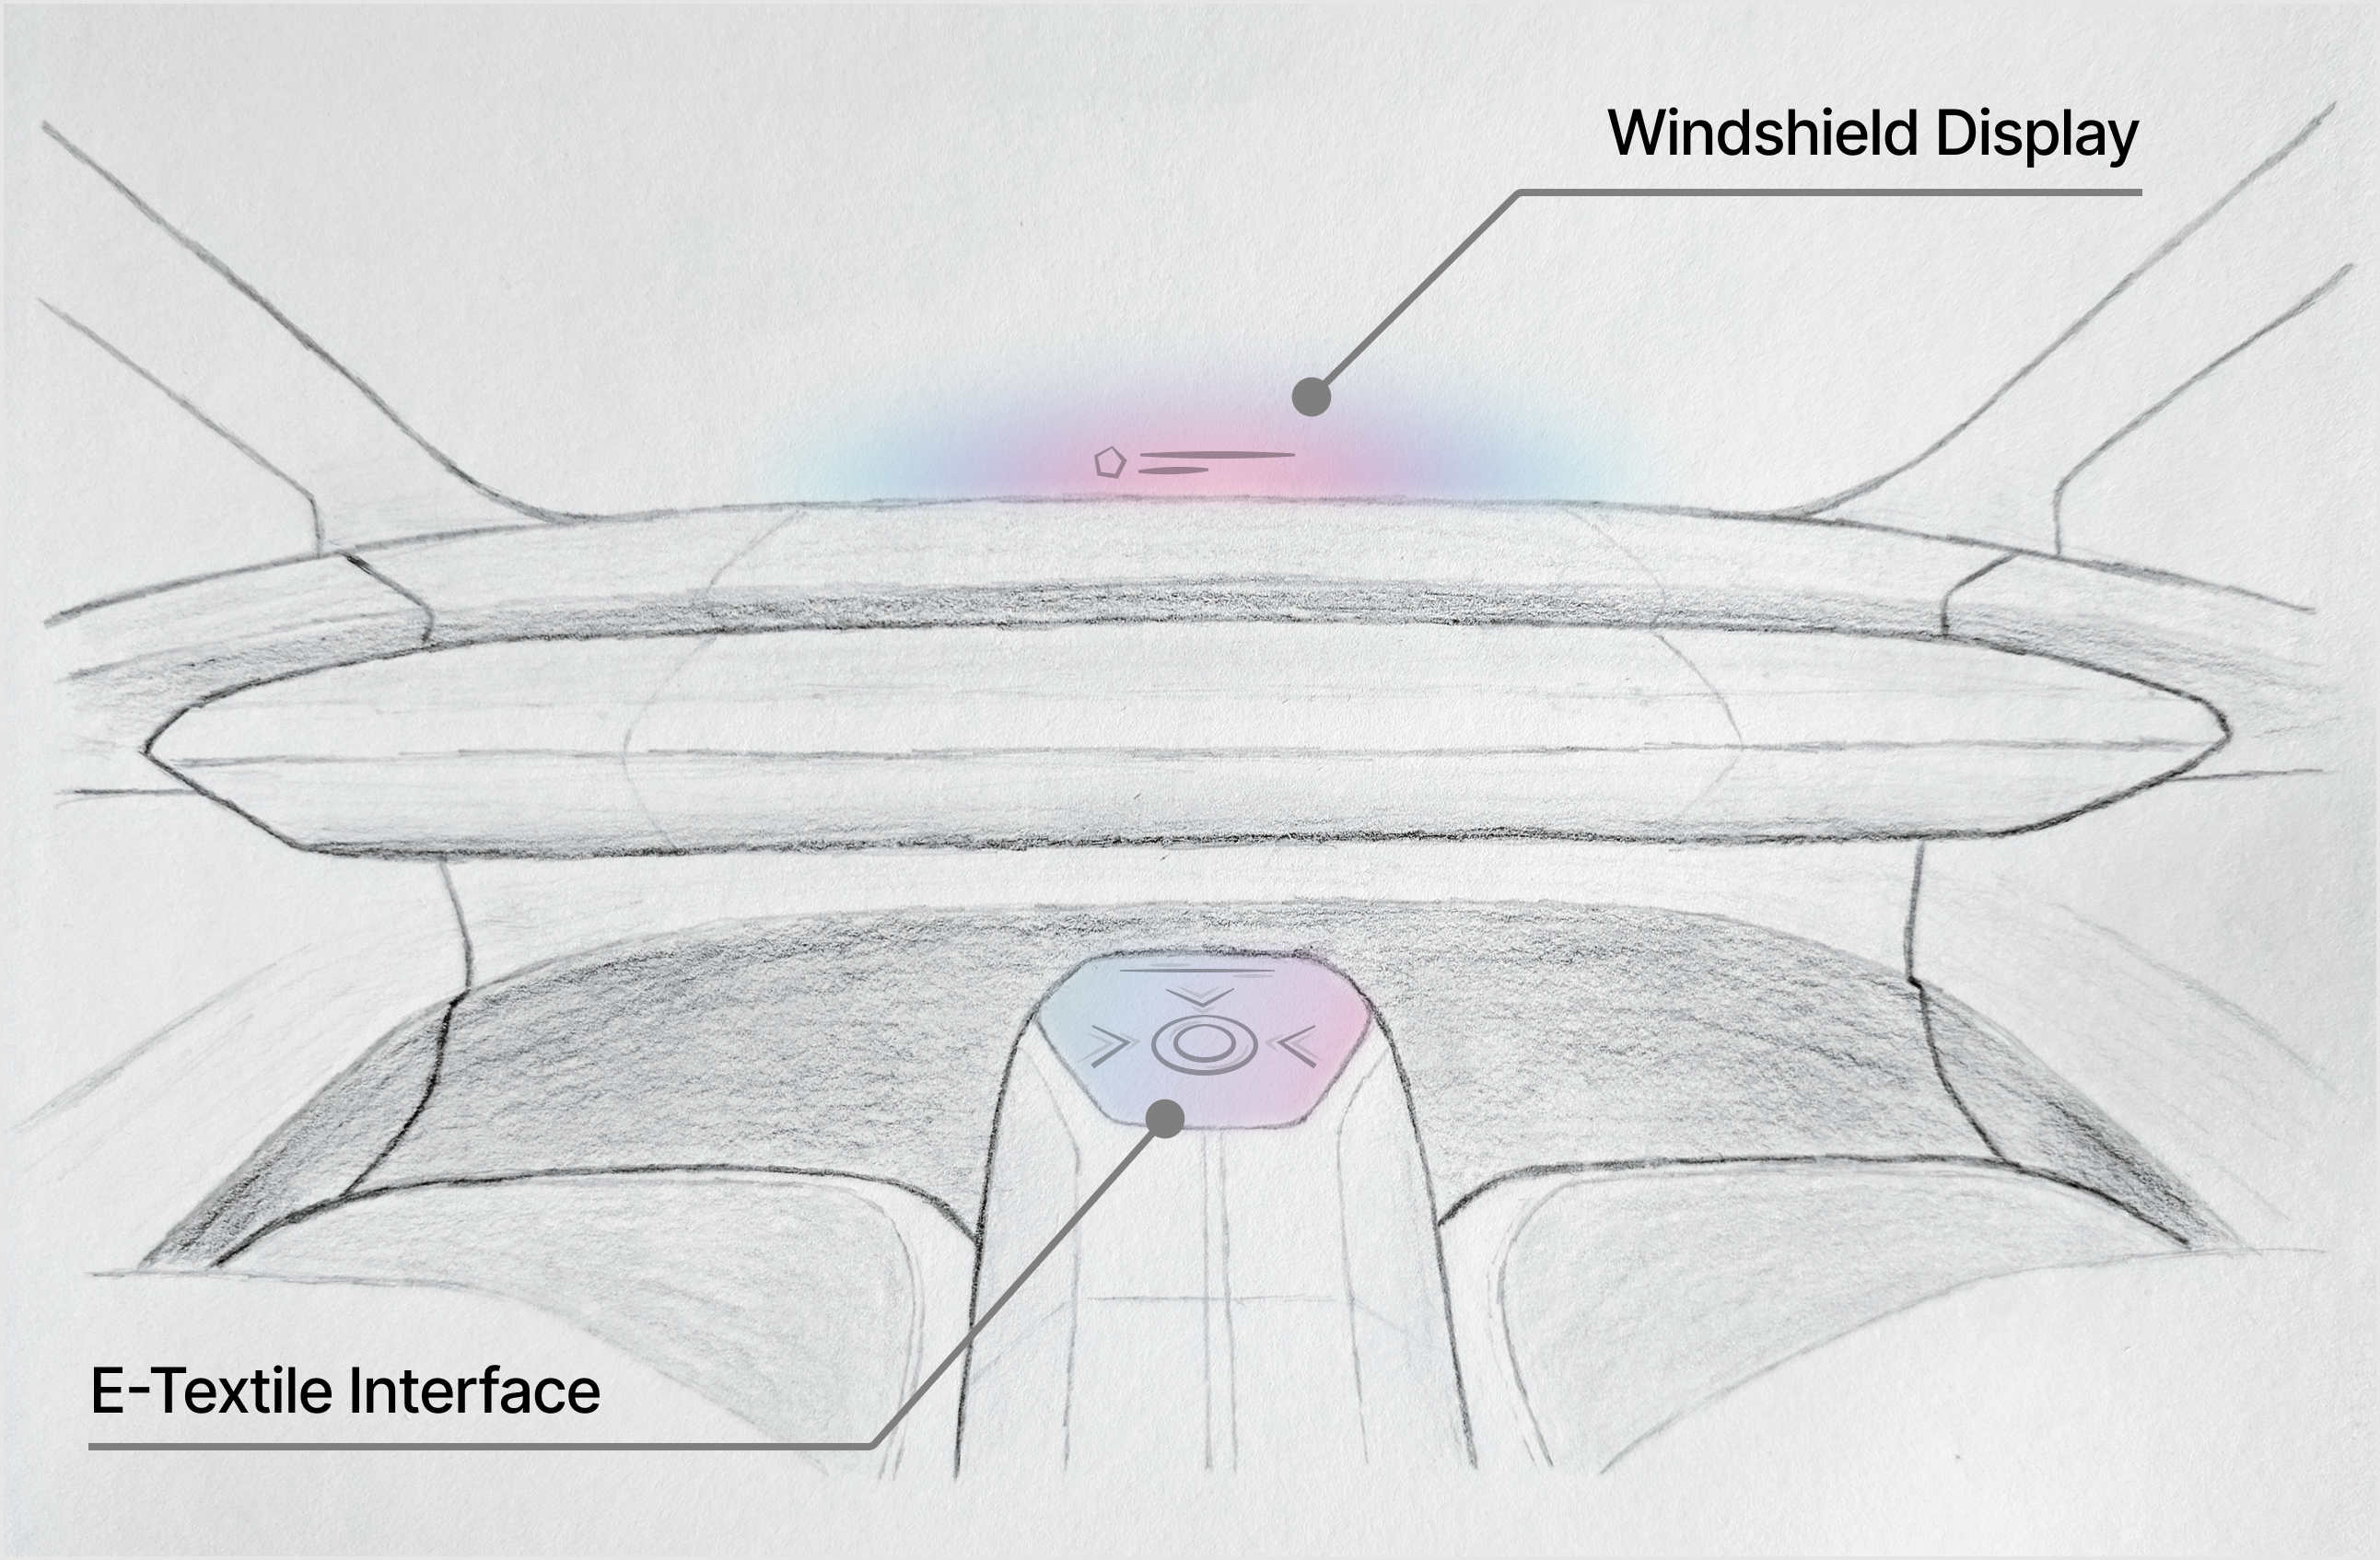
\includegraphics[width=1\linewidth]{images/Proposed Paradigm.png}
    \caption{Conceptual illustration of the proposed \gls{HMI} paradigm, combining a Windshield Display for visual output with an interactive e-textile surface for tactile input. Car interior based on the design of the BMW Neue Klasse concept \cite{bmw_neueklasse_2023}.}
    \label{fig:proposed_paradigm}
\end{figure}

The use of a \gls{WSD} as the primary visual output keeps the passenger's gaze directed forward, directly mitigating a primary cause of motion sickness \cite{diels_self-driving_2016}. As a complementary input method, an interactive e-textile surface can be integrated ergonomically on the center console armrest, while providing a natural and low visually demanding interaction with a hedonically appropriate tactile experience. Both technologies can be seamlessly and unobtrusively integrated, allowing for versatile and distraction-free \gls{NDRA}s while remaining aligned with the "living space" concept.
%By decoupling visual output from tactile input, this combined paradigm aims to create a more natural and less visually demanding interaction that addresses the key challenges of conventional interfaces.
% The use of a WSD as the primary visual output ensures that passengers can receive information without looking down and away from the direction of travel, directly mitigating a primary cause of motion sickness \cite{diels_self-driving_2016}. Furthermore when turned off it fully dispapers and alows the user to fully focus on NDRAs. Paired with this, an interactive e-textile surface for input addresses the remaining challenges. By embedding interaction into the soft, ubiquitous materials of the interior, e-textiles can be placed in ideal ergonomic locations, solving the "gorilla arm" problem \cite{berger_tactile_2019}. Unlike the "impersonal, digital, stiff, and cold objects" of today's devices \cite{brauner_interactive_2017}, the inherent warmth and rich textural properties of fabric align with the desired aesthetics of a "living space" and are better suited for "affective haptics communication" \cite{jiang_material-driven_2022}. Most importantly, the innate tactility of these interfaces provides the physical cues missing from featureless screens, creating the potential for a less visually demanding and more pleasant interaction experience.

\subsubsection{Windshield Displays}

A key component of the proposed \gls{HMI} paradigm is the use of the vehicle's windshield as the primary visual output. This concept is an evolution of the established \gls{HUD}, a technology initially developed for military aviation \cite{skirnewskaja_automotive_2022} and first introduced in cars by General Motors in 1988 \cite{weihrauch_first_1989}, that renders information in a partially-transparent display, allowing the user to comprehend it while still looking at the forward scene \cite{haeuslschmid_design_2016, skirnewskaja_automotive_2022}. The main advantage of \gls{HUD}s is that they are positioned close to the driver's natural line of sight, allowing information to be accessed quickly without the need to look down at the dashboard, thereby reducing the visual fatigue caused by switching between far and near perspectives \cite{haeuslschmid_design_2016, skirnewskaja_automotive_2022, zhu_value_2020}. While traditional \gls{HUD}s typically display limited, critical information like speed or navigation cues \cite{skirnewskaja_automotive_2022, weinberg_evaluating_2011}, the ever-increasing amount of information in modern vehicles requires new visualization concepts \cite{riegler_investigating_2018}.

One of the most promising solutions is the Windshield Display (\gls{WSD}), which Haeuslschmid et al. \cite{haeuslschmid_first_2016} describe as the "big siblings of head-up displays" that extend the display real estate to cover the entire windshield \cite{haeuslschmid_design_2016, hauslschmid_augmenting_2015}. \gls{WSD}s could be a critical component in the transition to automated vehicles by offering a multitude of benefits \cite{riegler_investigating_2018}. They can eliminate physical and visual clutter from the center console \cite{riegler_investigating_2018}, provide a single, unified interface for all in-vehicle systems \cite{gabbard_behind_2014}, and enable new gestural interaction modalities \cite{riener_gestural_2012}. The \gls{WSD}'s partial-transparency opens the door to a wide variety of Augmented Reality (\gls{AR}) applications, which could enhance in-vehicle experiences and further ease the transition from manual to \gls{HAD}  \cite{kun_arv_2017}. 

For highly automated vehicles, \gls{WSD}s have the potential to enhance user trust by increasing system transparency \cite{wintersberger_traffic_2017}.  For instance, a study by Wintersberger et al. \cite{wintersberger_traffic_2017} demonstrated that using an \gls{AR}-\gls{HUD} to create "traffic augmentation", highlighting other cars and potential hazards, significantly increased the participants' subjective feeling of trust in the automated system. Building on this, Lindemann et al. \cite{lindemann_catch_2018} demonstrated that an "explanatory windshield display", which visualizes the automation's reasoning and intended path, can significantly improve a passenger's situation awareness and understanding of the vehicle's behavior. 
 % However, the design of the information itself is crucial. Research by Dandekar et al., for instance, compared a WSD that used explicit pictograms against a more abstract, ambient light bar display around the windshield, while passengers engaged in NRDAs. They found that while both concepts successfully maintained high levels of trust and UX, the ambient light bar was actually preferred by users and provided a superior user experience, suggesting that less obtrusive, more integrated forms of information display may be more desirable than screen-based graphics, even when those screens are transparent \cite{dandekar_how_2022}.  

Beyond building trust, the \gls{WSD} can also directly influence the hedonic experience of the ride by transforming the journey itself into an engaging activity. For passengers in an \gls{AV}, a \gls{WSD} can display context-aware information, such as overlaying navigational aids onto the environment \cite{haeuslschmid_design_2016} or augmenting the view with information about points of interest \cite{haeuslschmid_first_2016}, effectively turning the act of sightseeing into an interactive learning experience \cite{matsumura_active_2018}. This directly caters to one of the possible primary \gls{NDRA}s in Avs, which is looking out the window and observing the environment \cite{ahram_what_2020, pfleging_investigating_2016}, also found to be a central factor for positive passenger experience in today's manually driven cars \cite{berger_designing_2021}. To further enhance this sense of exploration and fulfill the desires of active passengers, the \gls{WSD} could offer interactive functionalities. Passengers could, for example, zoom in on distant objects for a closer look, receive real-time translations of foreign signs, or "pause" the view to examine a fleeting scene in more detail \cite{matsumura_active_2018, pagura_window_2011}. 

The large display real estate also opens up new possibilities for entertainment and social connection. Researchers have explored concepts for in-car gaming \cite{togwell_-car_2022}, which could also invite to social interactions in the vehicle \cite{matsumura_active_2018}. This capability to support a wide range of \gls{NDRA}s is key to its potential to convert the vehicle into a true "infotainment platform" \cite{riener_automotive_2016}. Although the technology is still considered a young research field \cite{haeuslschmid_design_2016} and not yet commercially widespread due to technical, usability, and cost issues \cite{gabbard_behind_2014}, the potential can be easily evaluated in simulation \cite{riegler_investigating_2018}. Initial research has already produced several key design recommendations, addressing factors such as information placement preferences \cite{haeuslschmid_first_2016, riegler_investigating_2018}, optimal window background color and transparency \cite{riegler_adaptive_2019}, and the use of world-fixed versus screen-fixed positioning for displayed information \cite{riegler_stickywsd_2020}.

In essence, the \gls{WSD} provides a compelling solution for the visual output component of a future in vehicle \gls{HMI}. However a corresponding input modality is required to control the rich content on this new digital canvas, leading to the exploration of interactive textiles as a complementary solution.

% While the WSD provides a compelling solution for the system's visual output, the greater HMI challenge—and therefore the primary focus of this thesis—lies in the design of the tactile input modality. WSDs are an evolution of an established technology (HUDs), for which design recommendations already exist. Interactive textiles, by contrast, represent a novel paradigm for which the principles of intuitive interaction are still emerging. It is here, in the design of the physical interaction, that the core research questions of learnability, affordance, and feedforward must be addressed. Consequently, the remainder of this review will focus on establishing the state-of-the-art in designing these novel textile interfaces.


\subsubsection{Interactive E-Textiles}

While the \gls{WSD} offers a compelling solution for visual output, it requires a corresponding input modality that is ergonomic, unobtrusive, and hedonically aligned with the envisioned "living space". Interactive electronic textiles (e-textiles) present themselves as a uniquely suitable candidate to fulfill this role. 

Broadly defined, textile user interfaces are fabrics that can sense a user's physical interactions and produce responses as a result \cite{mlakar_exploring_2021}. By utilizing technologies like resistive and capacitive sensing, e.g. \cite{holleis_evaluating_2008, parzer_resi_2018, poupyrev_project_2016, goveia_da_rocha_crafting_2020, schneegass_gesturesleeve_2016, wu_project_2021, wu_zebrasense_2020}, they support a variety of versatile interaction methods that are comparable to those on conventional touch surfaces \cite{schafer_whats_2023}. The aim of research on interactive textiles is to "combine the power of digital devices with the ubiquity [and familiarity] of analog textiles" \cite[pp.~151]{brauner_interactive_2017}. By leaving the rigid shapes of today's devices behind \cite{castano_smart_2014, hamdan_sketchstitch_2018, posch_integrating_2018, poupyrev_project_2016}, e-textiles can extend the design space for \gls{HMI} and create novel input technologies that appeal to both visual and haptic perception \cite{mlakar_exploring_2021}.

%\paragraph{The Promise and Potential of E-Textiles}
\paragraph{The Potential of E-Textiles} \mbox{} \\
E-textiles offer a number of distinct advantages over conventional interfaces, particularly in addressing the pragmatic and hedonic limitations of touchscreens within the automotive context.

First, from an \textbf{aesthetic and tactile} perspective, textiles directly counter the "impersonal, stiff, and cold" materials like glass and plastic that dominate current in-vehicle interaction surfaces \cite{brauner_interactive_2017}. It is particularly attractive to overcome the boundaries between these traditionally rigid devices and soft, "human-facing materials" like fabrics \cite{olwal_e-textile_2020}.
Textiles are inherently perceived as warm, soft, and pleasant to the touch and come in a vast array of colors, forms, and structures \cite{brauner_interactive_2017}. This visual and haptic expressiveness \cite{hamdan_sketchstitch_2018} of the fabric itself is not merely decorative; combined with electronic components it provides the foundation for rich interactive experiences \cite{mlakar_design_2020} and better supports affective haptic communication \cite{jiang_gesfabri_2022}, as softer materials are consistently reported as more pleasant than stiff or coarse ones \cite{essick_psychophysical_1999}. This aligns perfectly with the goal of transforming the car into a comfortable and inviting living space \cite{schartmuller_automated_2020}.

Second, e-textiles excel in their potential for \textbf{seamless and ubiquitous integration}. This aligns with the foundational vision of ubiquitous computing, first articulated by Mark Weiser \cite{weiser_computer_1991}, which imagined computers that "weave themselves into the fabric of everyday life until they are indistinguishable from it" \cite[pp.~94]{weiser_computer_1991}. The goal is to achieve a state of "calm computing" \cite{case_calm_2015, denning_coming_1997}, where technology recedes from the foreground into our surroundings. 
%Because textiles are already omnipresent in vehicle interiors, embedding interactive functionality within them is a natural and less intrusive approach compared to artificial interfaces like touchscreens or remotes \cite{schafer_whats_2023, khorsandi_fabricar_2023}. Utilizing fabric and leather surfaces as seamless interfaces is a direct way to engage users in ubiquitous NDRAs and enrich their interaction with the environment (Khorsandi et al., 2023, p. 1439) 
Interactive textiles are a key enabler of this vision, aiming to "combine the power of digital devices with the ubiquity of analog textiles" \cite[pp.~151]{brauner_interactive_2017}. Because textiles are already a familiar, comfortable, and omnipresent material in vehicle interiors, they offer one of the most seamless, natural, and less intrusive ways of interacting with new technology \cite{brauner_interactive_2017, khorsandi_fabricar_2023, mlakar_exploring_2021, schafer_whats_2023}. With growing interest in such unobtrusive interfaces, everyday objects covered in smart textiles have the potential to become the "interfaces of the future" \cite{mlakar_design_2020}. They can thoroughly augment any object and provide "new and exciting features [...] that are difficult or impossible to realize with other solutions" \cite[pp.~1]{mlakar_design_2020}, allowing for the seamless and ubiquitous integration of controls and \gls{NDRA}s within the future car interior \cite{khorsandi_fabricar_2023}.

Third, the \textbf{physical form} of textiles offers significant ergonomic benefits. Unlike rigid electronics, textile-based devices can be shape-shifting, stretchable and bendable \cite{nanjappan_towards_2019}. This flexibility allows control interfaces to be placed in ideal ergonomic locations that are close to the passenger's body, such as on an armrest \cite{shishoo_textile_2008}, mitigating the arm fatigue associated with dashboard-mounted touchscreens \cite{berger_tactile_2019, sathyan_study_2020}. Furthermore, the material itself can be structured to provide inherent tactile guidance; for example, raised embroidery can guide a user's hand into the correct position without needing to look \cite{komor_is_2009}, a key advantage for reducing visual demand and potential motion sickness \cite{diels_self-driving_2016}. Fundamentally, these characteristics make textile interfaces an ideal medium for what Bakker and Niemantsverdriet \cite{bakker_interaction-attention_2016} call peripheral interaction. % In contrast to the focused interaction, such as demanded by touchscreens due required to visual attention, thus pulling attention away from NDRAs, a peripheral interface allows passengers to control vehicle functions without disrupting their primary task \cite{bakker_interaction-attention_2016}. 
Unlike touchscreens, which demand focused hand-eye coordination and can draw users away from their primary activity due to the required attention to interact, textile-based peripheral interfaces support unobtrusive vehicle interaction, allowing passengers to remain engaged in \gls{NDRA}s.
% In contrast to focused interaction, such as that required by touchscreens due to their high visual demand, peripheral interfaces enable passengers to control vehicle functions without diverting attention from their primary NDRA.

The importance of these hedonic qualities in driving user acceptance has been confirmed by empirical research. In a foundational study, Brauner et al. \cite{brauner_interactive_2017} evaluated user experience with an interactive motorized recliner armchair, directly comparing textile-based controls to a conventional plastic remote. Despite the remote control scoring higher on pragmatic qualities like efficiency, participants expressed a significantly higher preference and intention to use the textile interfaces. The study concluded that the primary driver for acceptance was the overall attractiveness and hedonic quality of the textile solution. Participants explicitly valued the "seamless integration of textile sensors into the design of the surrounding space" and the "cosiness of fabric", while criticizing the traditional remote as an "ugly" and "cold" element. This provides strong evidence that in a living space context, the aesthetic and material qualities of an interface can be more influential on user acceptance than its pragmatic performance.

%\paragraph{State of the Art and Application}
\paragraph{Current Applications} \mbox{} \\
The concept of interactive textiles is not new, as the field has been developing for over two decades, demonstrating its technological maturity. The modern era of e-textiles began in the late 1990s, when researchers like Post and Orth \cite{post_smart_1997} introduced techniques for embroidering interfaces with conductive thread and sensing touches through low cost capacitive circuits. 
%Since this pioneering work, a wide variety of fabrication methods have been developed, including weaving, knitting, and screen-printing conductive inks, allowing for the creation of robust and flexible touch-sensitive surfaces (Olwal et al., 2020, p. 2; Khorsandi et al., 2023, p. 1441). The technology has reached commercial viability, most notably with Google's Project Jacquard, which integrates conductive threads directly into fabrics on industrial looms (Brauner et al., 2017, p. 152).
Since this pioneering work, research has extensively explored the fabrication of various textile sensors. These methods generally fall into two categories: integrating conductive elements into standard textiles, or transforming the textile itself into a conductive fabric \cite{khorsandi_fabricar_2023}.

A wide variety of methods exist for integrating conductive threads and yarns, such as manual sewing or machine embroidery \cite{gilliland_textile_2010, hamdan_sketchstitch_2018, post_e-broidery_2000, goveia_da_rocha_crafting_2020, zeagler_textile_2012}, weaving \cite{pouta_woven_2022, wu_zebrasense_2020}, and knitting \cite{chen_design_2020, luo_knitui_2021}. Alternatively, fabrics can be made conductive through processes like coating non-conductive threads with metallic substances \cite{honnet_polysense_2020, lee_conductive_2015}, or by screen-printing conductive inks directly onto textile substrates \cite{goncalves_wearable_2018, zeagler_can_2013}. These techniques have enabled the creation of a diverse range of flexible sensors and interfaces \cite{olwal_e-textile_2020}, including touch matrices made from woven conductive thread \cite{parzer_resi_2018, parzer_flextiles_2016, poupyrev_project_2016} and multi-layer conductive fabrics \cite{leong_procover_2016, parzer_flextiles_2016, parzer_smartsleeve_2017, schneegass_gesturesleeve_2016}, thus preserving the shape-changing properties of conventional textiles. The technology has reached commercial viability, most notably with Google's Project Jacquard \cite{poupyrev_project_2016}, which incorporates conductive thread directly into fabrics on industrial looms to facilitate multitouch and gesture implementation. In fact, many recent approaches focus on creating \gls{2D} interactive surface patches \cite{leong_procover_2016, parzer_resi_2018, parzer_flextiles_2016, poupyrev_project_2016, schneegass_gesturesleeve_2016} that support gesture interfaces similar to modern multi-touch devices, enabling absolute \gls{2D} positioning, swipes, and even complex gestures like pinch-to-zoom \cite{olwal_e-textile_2020}.
%og location for consumer prutucts -> have been moved down

So far, research on e-textile interfaces has been largely dominated by two application domains: wearables \cite{heller_fabritouch_2014, jones_wearable_2020, karrer_pinstripe_2011, ono_textile_2017, parzer_smartsleeve_2017, schneegass_gesturesleeve_2016, strohmeier_zpatch_2018, yoon_timmi_2015} and smart furniture \cite{brauner_interactive_2017, heller_gardeene_2016, nabil_soft_2021, nabil_interioractive_2017, petersen_squeeze_2007}. Wearable applications leverage clothing to interact with devices \cite{nowak_shaping_2022}, with examples ranging from touchpads on trousers \cite{heller_fabritouch_2014} to gesture-sensing sleeves \cite{parzer_smartsleeve_2017}. In parallel, researchers have explored augmenting domestic environments by integrating controls into furniture, such as an armchair with embedded textile controls \cite{brauner_interactive_2017} or motorized curtains that can be opened and closed through touch gestures \cite{heller_gardeene_2016}.

However, despite the proven technical feasibility and potential applications, the transition to the consumer market has been challenging. Only a handful of products were developed using Google's Jacquard technology, such as the Levi's Commuter, Trucker, and Sherpa Jackets \cite{poupyrev_more_2017, poupyrev_smarter_2019}, as well as the Saint Laurent Cit-E \cite{poupyrev_smarter_2019} and Samsonite Konnect-I \cite{poupyrev_make_2020} backpacks. Furthermore, as of April 2023, Google discontinued the required Jacquard mobile app, rendering the core functionality of these products unusable \cite{bradshaw_google_2023}. This leaves a notable void in the market; to the best of our knowledge, there are currently no true consumer products featuring fabric with integrated touch-sensing capabilities, if one excludes smart home devices, like the Google Nest Mini \cite{google_store_google_nodate}, which often utilize conventional capacitive touch sensors placed underneath a passive fabric layer.


%\paragraph{Current Research Landscape for e-textiles for in-vehicle interaction}
\paragraph{Current Research Landscape on In-Vehicle E-Textiles} \mbox{} \\
Despite the opportunities presented by fabric-rich car interiors, there has been limited work at the intersection of e-textiles and \gls{HVI} \cite{khorsandi_fabricar_2023}. The existing research in this area can be broadly categorized. One line of work involves wearable physiological sensors integrated into jackets \cite{van_langenhove_smart_2004}, bracelets \cite{caon_wearable_2014}, or seat-belts \cite{wagner_16_2013} to detect the driver's biometrics, such as heart rate, breathing level, or concentration, with the vehicle adapting to passengers accordingly. Another area focuses on wearable devices for in-vehicle interaction, such as the fabric-based wrist-worn device by Nanjappan et al. \cite{nanjappan_towards_2019} controlling media and navigation through wrist and touch gestures. 
%While such wearable solutions offer intriguing possibilities for personalized control, this work intentionally focuses on non-wearable interfaces for several reasons. Requiring specialized clothing to interact with a car could be perceived as obtrusive by passengers and might present a barrier to adoption. It limits the interaction to only those wearing the specific garment, contrasting with the goal of creating a "walk-up-and-use" experience that is inherently shareable among all occupants of the vehicle.

Research on non-wearable textile surfaces, in line with our envisioned \gls{HMI} paradigm, is even more scarce. To the best of our knowledge, it is primarily limited to industry concepts like BMW's "Shy Tech" \cite{bmw_group_bmw_nodate}, academic posters \cite{khorsandi_functioning_2022}, and demonstrations \cite{dong_disappearing_2019} which often lack reported results from formal user studies. A notable exception is the work by Khorsandi et al. \cite{khorsandi_fabricar_2023} on FabriCar, which integrated textile sensors into a steering wheel, headrest, and seat-belt to study media control interactions. Their study made a significant contribution by demonstrating that textile interactions led to substantially less eye distraction compared to screen-based interactions during driving tasks.
% Old Ending:
% While this work validates the pragmatic potential of textile interfaces for reducing driver distraction, it leaves open the question of how to design such interfaces for the future context of autonomous vehicles, where the primary challenges shift from minimizing driver distraction to ensuring a hedonically rich and engaging user experience.

\paragraph{Summary} \mbox{} \\
While this work validates the technical feasibility and the pragmatic potential of textile interfaces, the primary challenges for the passenger-focused \gls{AV} context remain unaddressed. It is not yet clear how to design these novel surfaces to be immediately understood and effectively used by novice passengers, ensuring an experience that is not only hedonically rich but also fundamentally intuitive. Therefore, a deeper investigation into the principles of learnability and interaction guidance is required. 

% The ability to embed sensors ubiquitously into existing textile objects provides the advantage of creating simple control interfaces that are "less intrusive than other approaches" (Brauner et al., 2017, p. 152). This aligns with a design philosophy that moves toward minimalistic, aesthetically-integrated form factors that enrich our interaction with the existing environment (Khorsandi et al., 2023, p. 1439) [65, 79, 85]. When paired with a WSD that eliminates the visual clutter of a traditional dashboard, the e-textile input surface completes a holistic HMI that is both highly functional and unobtrusive. The result is an interface that supports the vision of "Interactive Interiors" (Nabil et al., 2017, p. 379) and moves the vehicle closer to the calm, integrated, and intuitive environment that the "living space" concept demands.


\subsection{Research Gap: Intuitive Interaction}

% Having established interactive textiles as a promising solution to the limitations of conventional in-vehicle interfaces, the central challenge now shifts from technological feasibility to interaction design. The very novelty of e-textiles is their primary hurdle: because most users have no established mental models for interacting with them, there is significant potential for confusion regarding where and how to perform an interaction. This presents a critical usability problem, as the HMI community shares the belief that such interfaces must not rely on training or explicit instructions to be used effectively.

Having established interactive textiles as a promising solution to the limitations of conventional in-vehicle interfaces, the central challenge now shifts from technological feasibility to interaction design. The very novelty of e-textiles is their primary hurdle: because most users have likely never encountered interactive textiles due to the lack of existing consumer products, they are not yet familiar with them \cite{mlakar_exploring_2021} and have yet to establish mental models for interacting with them, potentially leading to confusion regarding where and how to perform an interaction \cite{dong_disappearing_2019, mlakar_exploring_2021}. This presents a critical usability problem, as there is a shared belief in the \gls{HMI} community that "such interfaces must not rely on users getting training or explicit instructions or manuals to successfully interact with them" \cite[pp.~1159]{mlakar_exploring_2021}. To create such an onboarding-free "walk-up-and-use" experience, the interface itself must passively inform or remind the user about possible interactions \cite{mlakar_exploring_2021}. 
% This requires a deep understanding of how an interface can guide a user before they act.

The practical importance of this challenge is perfectly illustrated by comparing two early commercial products that used the same Google Jacquard \cite{poupyrev_project_2016} technology. The first product, the Levi's Commuter Jacket \cite{poupyrev_more_2017}, embedded an interactive area in the sleeve cuff (see Fig. \ref{fig:Levi's Commuter Jacket}). However, as Mlakar et al. \cite[pp.~1159]{mlakar_exploring_2021} critique, the jacket "does not [...] offer clear differentiation between the interactive and non-interactive area [...] nor does it give any indication of what actions are possible on that surface". This creates a situation where the possibility for interaction is effectively hidden, forcing a user to rely on a manual to know \textit{where} and \textit{how} to interact \cite{mlakar_exploring_2021}. In contrast, the Samsonite Konnect-I Backpack \cite{poupyrev_make_2020} used the same technology but with much more effective design. Its interactive strap clearly marks the interactive area through color and texture (see Fig. \ref{fig:Samsonite Konnect-I Backpack}). Its ribbed surface clearly suggests a sliding gesture, while its width hints that the interaction could be performed with a whole palm, instead of a single finger, providing an intuitive, built-in clue about how to interact \cite{mlakar_exploring_2021}. This comparison demonstrates that without deliberate design cues that make interaction possibilities obvious, even a technologically capable interface can fail in usability.

\begin{figure}
     \centering
     \begin{subfigure}[b]{0.49\textwidth}
         \centering
         \includegraphics[width=\textwidth]{images/Google Jacquard/Levi's Commuter Trucker Jacket.png}
         \caption{Levi's Commuter Jacket \cite{poupyrev_more_2017}}
         \label{fig:Levi's Commuter Jacket}
     \end{subfigure}
     \hfill
     \begin{subfigure}[b]{0.49\textwidth}
         \centering
         \includegraphics[width=\textwidth]{images/Google Jacquard/Samsonite Konnect-I Backpack.png}
         \caption{Samsonite Konnect-I Backpack \cite{poupyrev_make_2020}}
         \label{fig:Samsonite Konnect-I Backpack}
     \end{subfigure}
        \caption{Different implementation strategies of Google's Jacquard Technology \cite{poupyrev_project_2016} in consumer products.}
        \label{fig:Google's Jacquard Technology}
\end{figure}

% This comparison demonstrates that without the deliberate design of signifiers to create perceptible affordances, even a technologically capable interface can fail in usability.

%\subsubsection{The Learnability Problem: The Need for Intuitive Interaction}
\subsubsection{Learnability and the Need for Intuitive Interaction}

The ultimate goal for any novel interface is to achieve intuitive interaction. An intuitive interface is one that feels "easy" or "natural" to use, allowing a person to successfully operate it without undergoing a lengthy or effortful learning process \cite{mignonneau_designing_2005}. This sense of ease arises because the interaction effectively leverages a user's existing knowledge \cite{blackler_investigating_2010, khan_intuitive_2017}, both subconscious knowledge of physical affordances (e.g., buttons are for pressing) and conscious knowledge from past experiences or cultural conventions \cite{blackler_towards_2015}. In essence, intuitive interaction occurs when a user can immediately and non-consciously use an interface by drawing upon this stored knowledge \cite{chen_affordance_2017}.

This distinction is captured perfectly by Donald Norman's foundational concept of \textit{knowledge in the head} versus \textit{knowledge in the world} \cite{norman_design_2013}. "Knowledge in the head" is what we possess internally in our memory, such as learned skills and cultural conventions. "Knowledge in the world" refers to the information that is readily available and perceivable in our environment, such as visual signifiers, physical constraints, and natural mappings. While it is best when a user has considerable "knowledge in the head", a designer can place sufficient cues into the product itself, so that good performance is possible even without prior experience.

As Schäfer et al. \cite{schafer_whats_2023} note, the literature on textile interfaces is dominated by examples that require "knowledge in the head", forcing users to learn how a product works before use. Because most users have no prior experience with interactive textiles, they lack the stored "knowledge in the head" needed to interact intuitively. This creates a learnability gap, where the novelty of the interface prevents the natural, non-conscious interaction that users have come to expect from mature technologies. 
However, this challenge also presents a unique opportunity. Naumann et al. \cite{naumann_intuitive_2007} argue that aesthetics is the very gateway to intuitive use; it is the visual and tactile appeal of an object that invites a user to touch and explore, allowing them to then apply their prior knowledge. For novel interfaces, aesthetics can be "the key to the technology that lies behind" \cite[pp.~135]{naumann_intuitive_2007}.
Therefore, the central design problem is how to leverage the inherent aesthetic qualities of textiles and combine them with sufficient "knowledge in the world", guiding users toward correct interactions in a way that feels both intuitive and engaging \cite{schafer_whats_2023}.
% The central design problem, therefore, is how to bridge this gap by embedding sufficient "knowledge in the world" into the interface itself, guiding users toward correct interactions in a way that still feels intuitive.

% Herein lies the fundamental challenge for e-textiles: the very mechanism that enables intuitive use, which is a user's previous experiential knowledge, is precisely what is missing. As established, most users have no prior experience with interactive textiles and therefore lack the stored knowledge needed to interact intuitively. This creates a "learnability gap", where the novelty of the interface prevents the natural, non-conscious interaction that users have come to expect from mature technologies. The central design problem, therefore, is how to bridge this gap. If the interface cannot rely on a user's past, it must effectively teach them in the present, guiding them toward correct interactions in a way that still feels intuitive.

%\subsubsection{Feedforward as the Guiding Framework}
\subsubsection{Feedforward as a Guiding Framework}

% OG Feedforward Intro
\begin{comment}
    
% To understand how an interface can guide a user, it is helpful to analyze the interaction process itself. Any interaction between a person and a product can be seen as a continuous exchange of information. 
The primary way a designer can embed this "knowledge in the world" into an interface is by carefully considering the information exchanged between the product and the user.
This exchange can be broken down into what happens before, during, and after the user’s action \cite{vermeulen_crossing_2013}. The information the product provides during or after the user acts is commonly known as \textbf{feedback} \cite{wensveen_interaction_2004}. Wensveen et al. \cite{wensveen_interaction_2004} cite the dictionary definition of feedback  as "the return of information about the result of a process or activity" \cite{harpercollins_publishers_american_nodate}. For example, when a user pushes a power button to turn on a monitor, they receive feedback during the action: they feel the travel of the button and a "click" once it is fully depressed. After the action is complete, they receive further feedback when the screen lights up, confirming the result of their action.

However, a crucial part of the interaction happens before any action is taken. Before the user ever touched the button, the product had already offered information that communicated how it could be used. This information that is available before an action takes place is called \textbf{feedforward} \cite{wensveen_interaction_2004}. In the power button example, the fact that the button was protruding from its housing and was roughly the size of a fingertip served as feedforward, suggesting to the user that it could be pushed. While feedback confirms an action that has already occurred, feedforward makes the action discoverable in the first place.

To solve the learnability problem for novel interfaces with which users have no prior experience, thus no "knowledge in the head", the focus must therefore shift to this critical pre-interaction phase. While feedback is essential for a good user experience, it is the effective design of feedforward that makes a new system intuitively usable without any onboarding.
\end{comment}

The primary way a designer can embed this "knowledge in the world" into an interface is by carefully considering the information exchanged between the product and the user.
This exchange can be broken down into what happens before, during, and after the user’s action \cite{vermeulen_crossing_2013}. The information the product provides during or after the user acts is commonly known as \textbf{feedback} \cite{wensveen_interaction_2004}. Wensveen et al. \cite{wensveen_interaction_2004} cite the dictionary definition of feedback as "the return of information about the result of a process or activity" \cite{harpercollins_publishers_american_nodate}. For example, when a user pushes a power button to turn on a monitor, they receive feedback during the action: they feel the travel of the button and a "click" once it is fully depressed. After the action is complete, they receive further feedback when the screen lights up, confirming the result of their action.

However, a crucial part of the interaction happens before any action is taken. Before the user ever touched the button, the product had already offered information that communicated how it could be used \cite{wensveen_interaction_2004}. This pre-interaction guidance is provided by two related, but distinct, concepts: affordance and feedforward. 

The concept of affordance was coined by Gibson \cite{gibson_theory_1977}, and is described as all of the action possibilities that are present in the environment, independent of an individual's ability to recognize them. 
% In the context of HCI, Donald Norman \cite{norman_design_2013} adapted this concept to focus on perceived affordances: the aspects of a design that suggest to a user how the object should be used. Norman later argued that the term signifier is more accurate for these perceptible cues \cite{norman_way_2008}. The core function of a perceived affordance, or signifier, is to suggest how a user can physically interact with an object. For example a handle affords pulling, a button affords pushing, and a knob affords turning.
For design, the focus shifts to perceptible affordances, those possibilities for interaction that a user can correctly identify based on an object's design \cite{mlakar_exploring_2021}. William Gaver \cite{gaver_technology_1991} further refines this by categorizing affordances based on the alignment between perception and reality. Gaver referes to \textbf{perceptible affordances} as interaction possibilities that were correctly identified by users based on an object’s design. \textbf{Hidden affordances} are actual possibilities that are not perceived by the user, which can decrease usability, as was the case with the previously discussed Levi's Commuter Jacket \cite{poupyrev_more_2017} interactive sleeve. Conversely, \textbf{false affordances} are perceived possibilities that do not actually exist, leading to user error. As emphasized by Mlakar et al. \cite{mlakar_exploring_2021}, it is important to note that, following Gaver's definitions, an affordance only informs us about the possibilities for interaction (e.g., that a slider can be moved), not necessarily the function or result of that interaction (e.g., that moving the slider controls volume). The core function of an affordance is to suggest \textbf{\textit{how}} a user can physically interact with an object. For example a handle affords pulling, a button affords pushing, and a knob affords turning.

While affordances suggest possible actions, \textbf{feedforward} serves the distinct purpose of informing the user about \textbf{\textit{what will happen}} as a result of that action. As clarified by Vermeulen et al. \cite{vermeulen_crossing_2013}, this distinction is essential: an affordance reveals the \textit{physical action} and answers the question, "What can I do?", while feedforward reveals the \textit{functional result} by answering the question, "What will happen if I do it?". 

The power button example perfectly illustrates this synergy:
% \begin{figure} [h!]
%     \centering
%     \includegraphics[width=0.5\linewidth]{images/PXL_20250711_080025061.jpg}
%     \caption{Enter Caption}
%     \label{fig:enter-label}
% \end{figure}
\begin{itemize}
    \item Affordance: The button's protruding shape and size affords the physical action of pushing with a finger.
    \item Feedforward: A universal power symbol printed on it communicates that the result of pushing will turn on the device.
    \item Feedback: The tactile click and the screen lighting up confirm the action was successful.
\end{itemize}

This framework allows us to differentiate between the types of pre-action cues. Building on the foundational definitions by Wensveen et al. \cite{wensveen_interaction_2004}, which were later expanded by Vermeulen et al. \cite{vermeulen_crossing_2013} based on Hartson's expanded definition of affordance types \cite{hartson_cognitive_2003}, we categorize these cues as follows:

%Adapted from the foundational definitions by Wensveen et al. \cite{wensveen_interaction_2004} and the clarification by  Vermeulen et al. \cite{vermeulen_crossing_2013} based on Hartson`s \cite{hartson_cognitive_2003} expanded definition of affordance types, we categorize these cues as follows: 

\textbf{Inherent Feedforward Cues} are directly derived from the physical properties of an object and appeal to our perceptual-motor skills, such as the button's position, size and shape \cite{wensveen_interaction_2004}. This concept is closely aligned with the idea of physical affordance \cite{hartson_cognitive_2003}, as it communicates the information of possible interactions and how they can be carried out \cite{vermeulen_crossing_2013, wensveen_interaction_2004}. 

\textbf{Augmented Feedforward Cues}, by contrast, is information that comes from an additional source and appeals to a user's cognitive skills \cite{wensveen_interaction_2004}.
%(cognitive affordance)
% These cues are not built into the physical form in the same way as inherent feedforward cues, but they added on top to provide further guidance, revealing the function of an action. This can take the form of words, pictograms, or other signals like lights and sounds. A text label reading "Press to power on/off" next to the button or a pulsing light on the button symbolizing a chance to change the products power state are both examples of augmented feedforward.
These cues are not built into the physical form in the same way as inherent feedforward cues, but they are added on top to provide further guidance \cite{vermeulen_crossing_2013, wensveen_interaction_2004}. While these cues are often used to reveal the function of an action, e.g., a power symbol on a button \cite{vermeulen_crossing_2013}, we argue that they can also serve the critical purpose of clarifying an ambiguous or hidden physical affordance \cite{gaver_technology_1991, hartson_cognitive_2003}. This can take the form of words, pictograms, symbols or other signals like lights and sounds \cite{wensveen_interaction_2004}. For instance, a text label reading "Press to power on/off" next to the button or a pulsing light on the button are both examples of such augmented feedforward cues.

While Wensveen et al. \cite{wensveen_interaction_2004} and Vermeulen et al. \cite{vermeulen_crossing_2013} also describe a third category, functional feedforward, which informs the user about the general purpose of a product, the distinction between inherent and augmented feedforward is the most critical for analyzing the design of specific interface cues. This distinction provides the necessary framework to systematically investigate how different methods of embedding "knowledge in the world" can guide a first-time user.

% This aligns with the work of O'Brien et al., who argue that such feedforward techniques are essential for creating an intuitive interaction, as they guide the user’s "guessing process" by managing their expectations within a lenient learning environment where exploration is encouraged. 

% Ultimately, the effective use of these feedforward techniques is what enables intuitive interaction. O'Brien et al. support this view, defining intuitive HCI as interactions within "lenient learning environments" that allow a user to combine prior experience with feedforward methods to achieve their goals. They argue that designers can guide the user’s "guessing process" by using feedforward to manage their expectations about a system's response, making the interaction feel discoverable and predictable even for a novice user.

% This approach is central to enabling intuitive interaction, which O’Brien et al. define as a process where users effectively apply feedforward methods in a "lenient learning environment" to achieve their goals.

%\subsubsection{A Framework for Feedforward: The Feedforward Matrix}
\subsubsection{The Feedforward Matrix} \label{sec:feedforward-matrix}

While the distinction between inherent physical feedforward and augmented functional feedforward is useful, many cues in the real world are not so clearly defined. A cue can be partially integrated into an object's form, or it can simultaneously hint at both the action and the function. To systematically investigate how different cues guide a first-time user, a more nuanced framework is needed. Therefore, we propose a \textbf{Feedforward Matrix} (see Fig. \ref{fig:feedforward-matrix-empty}): a two-dimensional space that categorizes pre-interaction cues along two continuous axes.

\begin{figure} [h!]
    \centering
    \includegraphics[width=1\linewidth]{images/Feedforward Matrix/Feedforward Matrix Empty V2.png}
    \caption{The Feedforward Matrix, a two-dimensional framework for classifying pre-interaction cues based on their Integration Level and Information Type.}
    \label{fig:feedforward-matrix-empty}
\end{figure}

The first axis represents the \textbf{Integration Level}, describing how a cue is delivered in relation to the physical object. This is a spectrum ranging from Embedded/Inherent (where the cue is the physical form, such as its shape or texture) to Augmented/External (where the cue is an additional layer of information, such as a separate text label on a screen). An integrated LED light within a translucent button, for example, would fall somewhere in the middle of this spectrum; it is an augmented component, but it is physically part of the object's surface, making it feel more embedded than a separate instruction.

The second axis represents the \textbf{Information Type}, describing what kind of information the cue communicates. This is a spectrum based on the distinction clarified by Vermeulen et al. \cite{vermeulen_crossing_2013}. At one end is Affordance-Clarifying (action-focused), where cues answer the question, "What can I do and how?". At the other end is Function-Revealing (result-focused), where cues answer the question, "What will happen if I do it?". A cue can exist anywhere along this spectrum. For instance, the pulsing pattern of a light primarily clarifies an affordance ("interact here!"), but the presence of light itself carries a cultural association with electrical power, thus subtly revealing a potential function.

%\subsubsection{State of the Art in E-Textile Affordances and Cues / Emerging Design Principles for Tactile and Textile Interfaces}
\subsubsection{Feedforward and Affordances in E-Textiles}

Despite the technical maturity of e-textiles, many researchers \cite{jiang_gesfabri_2022, mlakar_exploring_2021, nowak_shaping_2022, schafer_whats_2023} note that the design of their interactive elements has received comparatively little attention. Much of the \gls{HMI} research in this area, as described by Schäfer et al. \cite[pp.~3]{schafer_whats_2023}, has focused on "questions of technical implementation and feasibility demonstrations". Mlakar et al. \cite[pp.~1160]{mlakar_exploring_2021} suggest this is a natural consequence of the field's early stage, where "technological innovation and fabrication are the main focus, and that the design of interactive elements is rarely a primary consideration when creating innovative prototypes". As a result, affordances or feedforward cues play a minor role in the current body of work on smart textile user interfaces \cite{mlakar_exploring_2021}, resulting in a lack of guidelines and recommendations regarding their design \cite{schafer_whats_2023}.

% This technology-driven focus has often led to a "bottom-up" design approach, where researchers first create a function and then find a matching gesture for it \cite{jiang_gesfabri_2022}. According to Jiang et al. \cite{jiang_gesfabri_2022}, the consequence of this approach is that the "relationship between the types of gestures and the affordance of the surfaces of e-textile received limited attention". This can result in interfaces that are not inherently intuitive and, as Mlakar et al. \cite{mlakar_exploring_2021} point out, often "require instructions to be understood", as the perceivable "knowledge in the world" is not available.

This technology-driven focus has often led to a "bottom-up" design approach, where researchers first create a function and then find a matching gesture for it \cite{jiang_gesfabri_2022}. Examples of such systems include RESi \cite{parzer_resi_2018}, which uses resistive yarn for tap and swipe gestures, FabricKeyboard \cite{wicaksono_fabrickeyboard_2017}, a deformable textile surface, and other interfaces designed for specific interactions like squeezing, e.g., Skweezee System \cite{vanderloock_skweezee_2013}, pinching, e.g., Pinstripe \cite{karrer_pinstripe_2011}, or grabbing folds of fabric, e.g., Grabrics \cite{hamdan_grabrics_2016}. According to Jiang et al. \cite{jiang_gesfabri_2022}, the consequence of this approach is that the "relationship between the types of gestures and the affordance of the surfaces of e-textile received limited attention". This can result in interfaces that are not inherently intuitive. For example, despite the high gesture recognition rate of the Skweezee System \cite{vanderloock_skweezee_2013}, participants found it difficult to form meaningful gestures on their own that were easy to remember and reproduce \cite{jiang_gesfabri_2022}. Similarly, the pre-defined behavior of Pinstripe \cite{karrer_pinstripe_2011} did not align with user expectations, particularly for a 'move forward' command in a menu \cite{jiang_gesfabri_2022}. As a result, such interfaces often require instructions to be understood \cite{mlakar_exploring_2021}, as the perceivable "knowledge in the world" is not available.

% However, a body of work is now emerging that shifts the focus toward deliberately designing well-understood physical affordances to support high usability and intuitive interaction \cite{jiang_gesfabri_2022}. This research has begun to produce initial design explorations with helpful insights \cite{mlakar_signifiers_2025, mlakar_exploring_2021, dong_disappearing_2019} as well as guidelines and recommendations based on user testing \cite{nowak_investigating_2025, schafer_whats_2023, nowak_shaping_2022, jiang_gesfabri_2022, mlakar_design_2020, brauner_interactive_2017} for textile interfaces.

However, a body of work is now emerging that shifts the focus from purely technical explorations toward deliberately designing user-centered textile interfaces. This research follows two complementary paths. One path focuses on establishing foundational guidelines for \textbf{haptic perception} \cite{mlakar_design_2020, nowak_shaping_2022, nowak_investigating_2025, schafer_whats_2023}, evaluating the recognizability of different shapes, profiles, and textures to support clear tactile guidance and eyes-free use. 
While these findings are critical for the practical construction of any tactile interface, the other stream of research focuses on how to leverage these physical properties to create \textbf{intuitive interactions}.  This research has begun to produce initial design explorations with helpful insights \cite{dong_disappearing_2019, mlakar_exploring_2021, mlakar_signifiers_2025} as well as guidelines and recommendations based on user testing \cite{jiang_gesfabri_2022, mlakar_design_2020} for textile interfaces.


\paragraph{Foundational Design Explorations} \mbox{} \\
A key example of this emerging focus on affordances is the design exploration presented in a pictorial by Mlakar et al. \cite{mlakar_exploring_2021}. The authors' stated goal was to move beyond a technology-driven approach and to systematically explore the design space of textile interfaces from a human-centered perspective. They sought to understand the "intricate relationship between the physical design of textile user interfaces [...] and how this changes users' perception of which gestures the interface supports" \cite[pp.~1160]{mlakar_exploring_2021}. To do this, an interdisciplinary team created and reflected upon a large collection of textile samples, exploring how different visual (shape, color) and haptic (texture, details) properties could communicate possibilities for interaction.

Their main contribution is a set of five clusters of findings and insights derived from this process. These insights highlight how specific design choices influence an interface's perceived affordances. For instance, they discuss how \textbf{ergonomics}, such as the size of an element or the shape of the surface beneath it, can suggest whether to interact with a single finger or a whole hand. They note that \textbf{visual affordances} are critical, as they provide the first hints for interaction, with color helping to create focus while shape is more important for communicating the required gesture. Furthermore, they explore the \textbf{perception of textures} and the innate \textbf{direction of movement} in fabrics, noting that some materials can afford sliding in one direction while resisting it in another, much like stroking a cat's fur. Finally, they advocate for an \textbf{economic usage of design elements}, warning that overloading an interface with complex haptics can lead to "haptic chaos" if not fabricated perfectly.

Crucially, Mlakar et al. \cite[pp.~1165]{mlakar_exploring_2021} present these findings as qualitative insights from their annotated portfolio and explicitly state that they "could not conduct a user study to formally evaluate [their] assumptions". This work therefore provides a rich vocabulary and a set of exploratory concepts for designing textile affordances, laying the groundwork for the more empirical, user-tested investigations that were to follow.

Building directly on this exploratory work, Mlakar et al. \cite{mlakar_signifiers_2025} would later shift their focus from surface gestures to more complex, "textile-specific interactions" such as pulling, twisting, folding, and knotting. 
This approach follows the strategy of "material-specific e-textile interaction design" proposed by Gowrishankar et al. \cite{gowrishankar_strategy_2017}, who argued that designers should derive interactions from the inherent physical properties and deformable qualities of the fabric itself, rather than simply replicating digital controls on a textile surface.
Using a Research through Design approach, they conducted a workshop where designers created 50 samples embodying these types of interactions, with a specific focus on identifying the \textbf{signifiers} used to communicate them to the user. The term "signifier" was proposed by Norman \cite{norman_way_2008} to describe intentionally placed cues that offer guidance on how to interact with the world, in contrast to affordances, which are the inherent action possibilities of a material or object.
The primary contribution of this work is the identification of three distinct categories of signifiers relevant to textile interface design. The first two, \textbf{Visual Signifiers} (e.g., color, shapes, graphics) and \textbf{Textile Signifiers} (e.g., textile contrasts, attributes and textures), confirm previously discussed design elements by research \cite{barati_affordances_2019, jiang_gesfabri_2022, mlakar_exploring_2021, mlakar_design_2020, nowak_shaping_2022, schafer_whats_2023}. However, the authors introduce a novel and important third category: \textbf{Staging Signifiers}. This category refers to how the interface is supported by its surrounding environment, such as the structure underneath it, its position and orientation in space, or the inclusion of non-textile materials that guide the interaction. For instance, providing the first step of an interaction (like a single tissue pulled from a box) or a protruding element underneath a textile surface suggesting to push it down are both powerful staging signifiers.

Beyond identifying these categories, the authors discuss observations from a user exploration session which revealed several key design considerations. They emphasize the \textbf{importance of visual perception}, noting that even for tactile interfaces, users tend to try and understand an interface visually before touching it. They also advocate for an \textbf{economic use of signifiers}, warning that using too many cues from different categories can lead to redundancy and unnecessary complexity. Perhaps most interestingly, they observed that signifiers that were familiar from other digital interfaces (e.g., arrows indicating direction) were more effective at communicating an interaction than associations with non-interactive everyday objects (e.g., an interface resembling a tissue box did not effectively communicate a "pulling" action). This suggests that even "natural" textile interactions may require clear, learned signifiers rather than relying solely on real-world metaphors. This work provides a rich, categorized vocabulary for intentionally designing cues for complex textile interactions.

% Another foundational exploration that specifically investigates feedforward for "disappearing" textile interfaces was conducted by Dong \cite{dong_disappearing_2019} in an automotive context. 
Bridging the gap between pure exploration and formal evaluation, the work by Dong \cite{dong_disappearing_2019} presents an early investigation of different inherent feedforward modalities for a "disappearing" textile interface in an automotive context. 
The work aimed to address the confusion users face when an interface is seamlessly embedded into a soft surface, such as a vehicle seat. The research designed and tested four different feedforward modalities for a simple volume adjustment task: a baseline with no feedforward, two visual cues (a static and a dynamic light pattern), and a physical, shape-changing cue. 

In a user test with 25 participants, Dong \cite{dong_disappearing_2019} found that the \textbf{shape-changing feedforward} was particularly expressive and effective at "triggering the users to interact with it". The physical nature of the shape-changing cue was noted to be easier to find and use via haptic perception, thereby reducing visual attention demand. The study's key finding was that a \textbf{combination of the shape-changing cue and the dynamic light pattern} presented the highest perceived affordance and resulted in the best user experience. 
% This early work is significant as it was one of the first to systematically compare different inherent feedforward modalities on a textile HMI, demonstrating a promising approach for designing more intuitive and enjoyable in-vehicle interfaces.
This work is significant as it represents one of the first attempts to systematically compare and empirically test different feedforward modalities on a textile \gls{HMI}, demonstrating a promising approach for designing more intuitive in-vehicle interfaces and paving the way for research focused on deriving user-tested guidelines.

\paragraph{User-Tested Guidelines and Recommendations} \mbox{} \\
A foundational study that empirically tested how physical forms afford specific interactions on non-wearable textile interfaces was conducted by Mlakar and Haller \cite{mlakar_design_2020}. While their research produced a number of guidelines for haptic design, its most relevant contribution for intuitive interaction was an experiment testing shape affordances. In this part of their study, participants were presented with simple, embroidered geometric shapes and asked to demonstrate how they would interact with them. The results confirmed that \textbf{the shape of an element can strongly afford a specific type of interaction}; for example, although all shared the same height of 13 mm, a vast majority of users intuitively chose to press on circular, square, and triangular shapes, while a 64 mm long rectangular shape was more ambiguous, affording both pressing and sliding gestures. This work provided early empirical evidence that designers can use simple, unambiguous geometric shapes to create predictable physical affordances on textile surfaces.

Shifting the focus from the geometry of specific widgets to the affordances of the material itself, Jiang et al. \cite{jiang_gesfabri_2022} explored how different textile textures can elicit intuitive gestures. Using a material-driven approach, they created five distinct textile textures (e.g., gathering, stuffed quilting, pleating) and conducted a gesture elicitation study to identify the "natural" gestures users would perform on each. Their study provided strong empirical evidence that \textbf{specific textile textures can indeed afford intuitive gestures with high user consensus}. For example, a "stuffed quilting texture" consistently afforded a poking gesture, while a "pleating texture" afforded stroking. A further key finding was the prevalence of single-handed gestures; based on their observations, the authors recommend associating single-hand gestures with e-textile interfaces to achieve higher intuitiveness. This work is significant as it validates the idea that the inherent properties of a material can be a powerful tool for designing intuitive interactions, a key principle in creating an interface that does not rely on pre-learned instructions.

%\paragraph{Summary/Key Findings/Gap?} 
\paragraph{Summary and Research Gap} \mbox{} \\
% Taken together, this body of work provides a strong and emerging foundation for valuable guidelines on how the inherent feedforward properties of a textile, such as its shape, profile, and texture, can be designed to create predictable physical affordances and elicit intuitive gestures. However, a critical analysis reveals a consistent focus throughout these studies: with the exception of Dong \cite{dong_disappearing_2019} they exclusively investigate inherent feedforward; the physical affordance cues of the textile itself. While this provides a strong foundation for designing the physical form of an interface, it leaves open the crucial question of how to best employ augmented feedforward, such as additional cues like light or sound, to guide users in more complex, multi-element scenarios.
Taken together, this body of work provides a strong and emerging foundation for designing textile interfaces. As illustrated in Fig. \ref{fig:feedfroward-matrix-focus}, it offers valuable initial guidelines on how the inherent physical properties of a textile, such as its shape and texture, can be designed to create predictable physical affordances and elicit intuitive gestures.
However, a critical analysis reveals that the existing research has almost exclusively focused on single interaction elements in isolation, with each element typically affording only a single, predefined interaction. This approach falls short of addressing the need for more complex surfaces for in-vehicle \gls{HMI} that require multiple context-dependent controls. Moreover, while these studies provide a foundation for designing the physical form of an interface (inherent feedforward), they leave open the crucial question of how to best employ augmented feedforward, such as light, to guide users. Even in the rare cases where augmented cues were explored, as in the work by Dong \cite{dong_disappearing_2019}, their purpose was limited to clarifying the physical action (e.g., 'interact here by sliding'). To date, no work has systematically investigated how augmented feedforward can communicate the functional result of an interaction on textile (e.g., 'this slider controls volume'). Therefore, it remains unclear how different levels of feedforward, ranging from inherent physical properties to augmented visual cues, can be combined to guide first-time users in discovering not only how to interact with a textile interface, but also what they can achieve by doing so.

\begin{figure}[h!]
    \centering
    \includegraphics[width=1\linewidth]{images/Feedforward Matrix/Feedforward Matrix Gap.png}
    \caption{The Feedforward Matrix, illustrating the current research focus on textile user interfaces.}
    \label{fig:feedfroward-matrix-focus}
\end{figure}


\subsection{Summary} % Summary and Relevance to this work??

The reviewed literature highlights a profound shift in the role and expectations of future vehicle interiors, driven by increasing levels of automation. As passengers become disengaged from the driving task, vehicle cabins are transforming into multifunctional living spaces that must support a diverse array of \gls{NDRA}s, which researchers identified ranging from passive relaxation to cognitively demanding tasks. This transformation introduces new challenges for in-vehicle \gls{HMI}s, particularly in terms of ergonomics, usability, and hedonic quality.

Touchscreen-based interfaces, while widespread, have been found to suffer from significant limitations in this context, including high visual demand, poor ergonomics in motion, and a lack of tactile or emotional appeal. In contrast, interactive e-textiles have emerged as a promising alternative, offering a combination of material familiarity, aesthetic richness, ergonomic flexibility, and seamless integration with the vehicle environment, while enabling low-attention, peripheral interaction. When paired with \gls{WSD}s, these textiles can create a novel \gls{HMI} paradigm, aligning with both pragmatic and hedonic user needs highlighted by researchers in the \gls{AV} context, which are found to be crucial for the success of the \gls{HAD} technology.

However, while the technical feasibility of e-textile interfaces has been demonstrated in numerous publications, there remains a notable lack of research applying them to function-rich, in-vehicle \gls{HMI} or exploring how they can be designed for intuitive use. The literature emphasizes that to achieve an intuitive "walk-up-and-use" experience, the interface itself must provide the necessary cues through "knowledge in the world" to guide the user. Recent research has begun to address this by exploring how the inherent physical properties of a textile, such as shape and texture, can create predictable physical affordances. While this work provides good foundational guidelines to implement inherent feedforward  in single textile interaction elements, research on multi-element interfaces and the role of augmented feedforward cues remain unexplored.

This analysis reveals a crucial research gap. There is a lack of studies that holistically examine different levels of feedforward, from inherent to augmented and from seamlessly integrated to explicit cues, particularly in the context of non-wearable textile interfaces embedded in vehicle interiors.
Beyond the need for intuitiveness, a crucial and neglected aspect is the intentional design of these interfaces to create positive, engaging experiences. The current body of work does not adequately address how to design textile \gls{HMI}s that support the diverse needs of future passengers while prioritizing these vital hedonic qualities for acceptance of \gls{AV} technology. 
% This gap is significant; beyond the need for intuitiveness, a crucial and neglected aspect is the intentional design of these interfaces to create positive, engaging experiences. The current body of work does not adequately address how to design textile HMIs that support the diverse NDRA needs of future passengers while prioritizing these vital hedonic qualities. 
% This gap becomes even more pronounced considering that besides the need for interfaces that are intuitive for first-time users a crucial aspect that has been neglected so far which is designing textile in-vehicle interfaces intentionally to creating  positive experiences through interaction while supporting the diverse NDRA needs within the vehicle HMI of future passengers.
% Beyond the need for intuitive interaction, existing research also largely neglects the hedonic dimension: how such interfaces can be designed to create emotionally engaging and pleasing experiences. This is particularly important given the central role of positive user experience in shaping the acceptance of AV technology.
 
To address this gap, this work investigates how different levels of feedforward can support intuitive, walk-up-and-use interactions with a non-wearable textile interface designed for \gls{NDRA}s in \gls{AV}s. The central research goal is to identify which level of feedforward best balances intuitiveness with a novel and emotionally engaging user experience, 
% enabling richer, more accessible interactions within the emerging paradigm of textile-based in-vehicle HMIs.
thereby contributing to the development of expressive, user-centered textile \gls{HMI}s for future vehicle interiors.

% oldest version
\begin{comment}
    This Feedforward Matrix provides a powerful tool for analyzing interfaces and identifying precise gaps in the research literature. Much of traditional product design has focused on the "Embedded, Affordance-Clarifying" space (i.e., traditional physical affordances). In contrast, many graphical user interfaces rely on the "Augmented, Function-Revealing" space (i.e., explicit icons and text labels).

    However, for novel materials like interactive textiles—which lack both the established affordances of traditional physical objects and the conventional symbolic language of screens—a significant gap in understanding emerges. It is unclear how designers can best utilize cues that fall between these extremes. Specifically, there is a lack of systematic investigation into how different types of augmented, affordance-clarifying cues (such as dynamic lights or simple instructional text) impact the intuitive use, learnability, and overall user experience for first-time users of non-wearable e-textile interfaces.

    This thesis aims to address this gap directly. By systematically designing and evaluating interface variations that occupy different positions within the Feedforward Matrix, this work seeks to understand how to best embed "knowledge in the world" to create an onboarding-free and engaging experience for the passenger of the future.
\end{comment}

% old version
\begin{comment}
    

% The body of work reviewed above provides a strong and emerging foundation for the design of tactile textile interfaces. Through rigorous user testing, we now have clear, evidence-based guidelines. We know that raised profiles are more effective than flat ones for haptic recognition (Schäfer et al., 2023), that recessed sliders provide excellent guidance (Nowak et al., 2022), that simple geometric shapes are key for recognizability (Mlakar \& Haller, 2020), and that the inherent texture of a material can afford intuitive gestures (Jiang et al., 2022).

% However, a critical analysis of this literature reveals a significant gap. These studies, with few exceptions, focus almost exclusively on inherent feedforward—investigating the physical affordances of a single textile element in isolation. This research primarily answers the question, "What can I do with this object?". It does not address the equally important question for any real-world system: "What will happen if I do it?".

% For a complex, multi-element control surface, such as that required for an in-vehicle HMI, relying on inherent cues alone is insufficient. When multiple interactive elements are placed together, their physical affordances can compete, potentially creating confusion. More importantly, the user has no way of knowing which tactile element is connected to which system function. This is precisely the scenario where augmented feedforward—additional cues like light or sound—becomes critical, not just to clarify the action, but to reveal its function.

% Using the Feedforward Matrix proposed earlier, we can precisely locate this gap. While existing research provides valuable guidelines for the "Embedded, Affordance-Clarifying" quadrant of the matrix, the design space for augmented feedforward in textile interfaces remains largely unexplored. Specifically, there is a clear lack of research that systematically investigates and differentiates how various levels of augmented cues (from seamlessly integrated lights to more explicit symbols) impact not just the functional usability, but the full user experience—including perceived intuitiveness, hedonic qualities, and emotional response—in the context of complex, non-wearable textile interfaces for autonomous vehicles.

% This thesis aims to fill this critical gap. By systematically designing and evaluating interface variations that occupy different positions within the Feedforward Matrix, this work seeks to understand how to best embed "knowledge in the world" to create an onboarding-free and engaging experience for the passenger of the future.
\end{comment}


% affordance mess
\begin{comment}
    
The term, originally coined by Gibson, describes how the properties of an object or environment make particular actions possible for an individual who can perceive them. In the context of HCI, the concept has been further developed to describe the "design aspect that offers or provides visual cues to the user on using a physical artifact" (Jiang et al., 2022, p. 2). Gaver (1991) further refines this by distinguishing between different types of affordances. When interaction possibilities are correctly identified by a user based on an object's design, they are called perceptible affordances. If these possibilities exist but are not perceivable by the user, they become hidden affordances, which decreases usability. Conversely, if the design implies an interaction is possible when it is not, it creates a false affordance (Mlakar et al., 2021, p. 1160). Crucially, an affordance only informs the user about the possibility of an interaction (e.g., a slider's shape affords linear motion), not necessarily its function (e.g., controlling volume) (Mlakar et al., 2021, p. 1160).

----

To use feedforward as an effective design framework, it is crucial to differentiate between its types. Wensveen et al. (2004) provide a useful distinction based on where the information originates and what cognitive skills it appeals to. However, to fully grasp this distinction, one must first understand the related concept of affordance.

The term was originally coined by the psychologist James Gibson \cite{} and later adapted for the field of Human-Computer Interaction (HCI). An affordance refers to the properties of an object that show a user the actions they can take. As Gaver (1991) elaborates, affordances are "properties of the world that are compatible with and relevant for user interaction". Crucially, affordances must be perceivable to be effective. When interaction possibilities are correctly identified by a user based on an object's design, they are called perceptible affordances; otherwise, they are hidden affordances that decrease usability. An affordance informs the user about the possibility of an action (e.g., a handle affords pulling) but not necessarily its function (e.g., that pulling the handle will open a door). With this understanding, we can now differentiate the types of feedforward.


---
\end{comment}

% affordance mixed with feedforward to brindge the gulf of execution
\begin{comment}
    To understand how feedforward can be designed to solve the learnability problem, it is crucial to clarify its relationship with the foundational concept of affordance. While often used interchangeably, and both essential for bridging what Norman calls the "Gulf of Execution" , they serve distinct purposes.


The most effective way to disambiguate them is by the question they answer for the user. A perceived 


affordance answers the question, "What can I do?". It reveals the physical action possibilities of an interface—that a button can be pushed, a knob can be turned, or a textile can be swiped. 


Feedforward, on the other hand, answers the question, "What will happen if I do it?". It reveals the purpose or result of that action, telling the user that pushing the button will submit a form or that swiping the textile will adjust the volume. An interface is only truly intuitive when it successfully communicates both.


The framework by Wensveen et al. (2004), which distinguishes between inherent and augmented feedforward, can be understood through this lens.

Inherent Feedforward primarily communicates the affordance ("What can I do?"). It is information derived from the physical form of the product itself, appealing to a user's perceptual-motor skills. It communicates what kind of action is possible—such as pushing, rotating, or sliding. In our power button example, its physical protrusion and shape afford "push-ability", which is a form of inherent feedforward.

Augmented Feedforward primarily communicates the feedforward ("What will happen?"). It is information from an additional source that is layered on top of the physical form and appeals to a user's cognitive skills. This can take the form of words, pictograms, or other signals like lights and sounds. A text label reading "Power" next to the button or a glowing light that pulses to draw attention to it are both examples of augmented feedforward, as they reveal the function of the interaction.

This distinction between physically inherent cues that communicate the possible action, and cognitively augmented cues that communicate the resulting function, provides the necessary framework to systematically investigate how different methods of embedding "knowledge in the world" can guide a first-time user



To understand how feedforward can be designed to solve the learnability problem, it is crucial to differentiate between its types. This distinction, however, first requires an understanding of the related, foundational concept of affordance.
\end{comment}

% affordance-free version (backup)
\begin{comment}
Feedforward is not a monolithic concept. To use it effectively as a design framework, it is crucial to differentiate between its types. Wensveen et al. \cite{wensveen_interaction_2004} provide a useful distinction between inherent and augmented feedforward, based on where the information comes from and what cognitive skills it appeals to.

% is directly related to the physical properties of a product and how they invite a certain action, without any extra labels or instructions, appealing primarily to a user's perceptual-motor skills. 
\textbf{Inherent Feedforward} is directly related to the physical properties and action possibilities of a product, appealing primarily to a user's perceptual-motor skills. It is the information that communicates what kind of action is possible, such as pushing, rotating, or sliding, and how that action can be carried out. Wensveen et al. \cite{wensveen_interaction_2004} note that inherent feedforward can be seen as a specific interpretation of the concept of affordance, where the focus is on the action possibility of the control itself, regardless of its ultimate function. In our power button example, its protrusion, shape, and size, which suggest "push-ability", are forms of inherent feedforward.

\textbf{Augmented Feedforward}, by contrast, is information that comes from an additional source and appeals to a user's cognitive skills. It is not built into the physical form in the same way, but is added on top to provide further guidance. This can take the form of words, pictograms, or other signals like lights and sounds. A text label reading "Push to power on" next to the button or a glowing light that pulses on the button to draw attention to it are both examples of augmented feedforward.

While Wensveen et al. \cite{wensveen_interaction_2004} also describe a third category, functional feedforward, which informs the user about the general purpose of a product, the distinction between inherent and augmented feedforward is the most critical for analyzing the design of specific interface cues. This distinction provides the necessary framework to systematically investigate how different methods of embedding "knowledge in the world" can guide a first-time user.
\end{comment}


% as the textile is the main touchpoint the focus lays on it's design (but the WSD isn't fully neglected of course)


% \subsubsection{Identifying the Specific Research Gap}
% This is the climax of your literature review. Argue that while prior work has touched on textile affordances or cues, it has not systematically investigated or differentiated how various levels of feedforward (inherent vs. augmented) impact the full user experience—including perceived intuitiveness, hedonic qualities, and emotional response—in the context of complex, non-wearable textile interfaces for autonomous vehicles.





\begin{comment}
***My own limitation kind of*** 
“we did not limit ourselves by the sensor technology but focused more on tactile perception and active user interaction” [Mlakar and Haller, 2020, p. 2]
\end{comment} 

%% HAPTIC DESIGN GUIDELINE GRAVEYARD ++++ REVIVE FINDINGS IN PROTOTYPING SECTION %%
\begin{comment}

Mlakar & Haller (2020) --------------------------------------------
A foundational study that systematically derived guidelines for the design of non-wearable textile interfaces was conducted by Mlakar \& Haller \cite{mlakar_design_2020}. Their research followed a multi-stage process, beginning with initial design assumptions derived from industry partnerships, which were then refined through interviews with six design experts. Finally, they conducted a user study with 30 participants to empirically test five key statements about the eyes-free tactile recognition of embroidered elements. The study resulted in five clear design recommendations that provide a baseline for creating perceivable tactile interfaces. The authors found that using \textbf{explicit contrast} is crucial for differentiating elements, with \textbf{height contrast} being the most effective and easily recognized cue, followed by shape, and finally texture. They also established recommendations for size, finding that tactile shapes should be no smaller than 6.5 mm, with an \textbf{optimal size of 13 mm or larger} for reliable recognition. The research confirmed that the \textbf{shape of an element can strongly indicate the required interaction}, for example, a circular bump affords pressing, while a straight line affords sliding. A key finding was that designers should \textbf{keep shapes as simple as possible}, as the study revealed that common visual UI symbols (like a star or a phone icon) are extremely difficult to recognize by touch alone. This work provides some of the first concrete, user-tested guidelines for designing the fundamental building blocks of tactile textile interfaces.

Nowak et al. (2022) -----------------------------------------------
%Building on foundational work on textile elements, Nowak et al. \cite{nowak_shaping_2022} conducted a deep dive into the specific design of one crucial interaction element: the textile slider. 
Following earlier work on general interactive elements, Nowak et al. \cite{nowak_shaping_2022} addressed the need for more specific guidelines by focusing on a single, complex component: the textile slider. Through two separate user studies, they systematically evaluated how different form factors and tick mark designs affect user performance and preference during eyes-free interaction. Their research provides a set of concrete, evidence-based guidelines for this common interactive component. Their first study investigated the fundamental shape and profile of sliders. A key finding was that \textbf{recessed sliders}, which create a physical groove for the user's finger, provided significantly better guidance and comfort than flat or raised sliders, whose paths were difficult to follow without looking. Their second study focused on the role of tick marks for eyes-free orientation and value selection. The results showed that \textbf{tick marks were more effective than the overall slider shape} (e.g., a curve) at helping users confidently determine their position. The study recommends using \textbf{at least three tick marks} to significantly improve selection accuracy over a blank slider. Furthermore, they found that specific tactile designs for tick marks (such as rotating or elevating them) could help users orient themselves with less exploratory hand movement. This work represents a significant step in developing a practical design vocabulary, providing specific, user-tested recommendations for a core textile widget.

Schäfer et al. (2023) & Nowak et al. (2025) -------------------------
%long version
To better understand the principles of creating distinguishable tactile elements on fabric, Schäfer et al. \cite{schafer_whats_2023} conducted a large-scale study on the haptic recognition of different textile shapes to derive clear design guidelines. They empirically tested 84 tactile elements, varying their shape, height profile (raised, recessed, or flat), and fill (filled vs. outlined) in an eyes-free recognition task.
The study's most critical finding was the dramatic impact of the element's physical profile. 
\textbf{Raised profiles} consistently outperformed all other haptic icon variants, yielding the highest success rates, the fastest recognition times, and the most positive user ratings for confidence and comfort. In contrast, flat elements that relied only on the texture of the embroidery were not reliably identifiable by touch alone. Furthermore, their work confirmed the importance of \textbf{simplicity in shape design}, as participants struggled to recognize complex visual symbols by touch alone. This research provides core, evidence-based principles for designing haptically perceivable and distinguishable elements on textile surfaces.

Building directly on the findings for single textile icons, Nowak et al. \cite{nowak_investigating_2025} investigated the next logical question: how does the presence of a neighboring icon affect haptic recognition? While previous work established guidelines for individual icons, practical interfaces consist of groups of controls placed near each other. To explore this, the authors conducted a user study where participants performed an eyes-free recognition task on pairs of raised textile icons, and also rated how easy the icons in each pair were to tell apart. The study's primary finding was that users did not benefit from having a neighboring icon for comparison. The recognition rate and time for a specific icon remained relatively consistent regardless of the icon it was paired with. This suggests that users were not effectively using the features of one icon to help identify another. The key implication of this work is a crucial design guideline for textile layouts: designers cannot rely on context or relative comparison to make tactile elements more recognizable. Instead, each individual element in a textile interface must be designed to be robustly and unambiguously identifiable on its own. This study adds a critical layer of understanding for the layout and composition of textile interfaces, highlighting the challenges of designing more complex, multi-element control surfaces.

A specific focus within this research has been on the challenge of eyes-free haptic recognition, which provides foundational principles for designing purely tactile cues. Schäfer et al. \cite{schafer_whats_2023}, for example, conducted a large-scale empirical study to derive clear design guidelines for tactile shapes. Their most critical finding was that an element's physical profile has a dramatic impact on its recognizability, with raised profiles consistently outperforming flat or recessed ones in speed, accuracy, and user confidence. Building directly on this, Nowak et al. \cite{nowak_investigating_2025} investigated the next logical step: how recognition is affected when these tactile elements are placed next to each other in pairs. Their key finding was surprising: users did not benefit from having a neighboring element for comparison, and the recognition rate for any given shape remained consistent regardless of its neighbor. Taken together, these studies provide crucial, evidence-based guidelines for designing distinguishable tactile elements, emphasizing that for haptic interaction, designers should prioritize raised profiles, simple geometric shapes, and ensure that each element is unambiguously identifiable on its own, rather than relying on context or relative comparison.

\end{comment}


